\documentclass[11pt]{article}

% AMS Packages
\usepackage{amsmath} 
\usepackage{amssymb} 
\usepackage{amsthm}
% Page dimensions
\usepackage[margin=1in]{geometry}
% Images
\usepackage[pdftex]{graphicx} 
% Enumerate package
\usepackage{enumitem} 
\usepackage{array} 
% Fancify pages
\usepackage{fancyhdr} 
% Convert captions on figures to bold font
\usepackage[labelfont=bf,textfont=md]{caption}
% Time New Roman font
\usepackage{times}
\usepackage{setspace} 
% si units in latex
\usepackage{siunitx}
\usepackage{textcomp} 
% Change sizes of sections
\usepackage{titlesec}
\titleformat{\section}{\normalfont\Large\bfseries}{\thesection}{1em}{}
\titleformat{\subsection}{\normalfont\bfseries}{\thesubsection}{1em}{}
\titleformat{\subsubsection}{\normalfont\small\bfseries}{\thesubsubsection}{1em}{}
% Declare useful math operators
\DeclareMathOperator*{\argmin}{arg\,min}
\DeclareMathOperator*{\plim}{plim}
\DeclareMathOperator{\Tr}{Tr}
\usepackage{graphics}

\usepackage{biblatex}
\addbibresource{ndbib.bib}

\usepackage{tikz}
\usetikzlibrary{shapes.geometric, arrows}
\usepackage{float}

% title
\title{Heterogeneous synaptic weighting enhances encoding and decoding in the presence of common noise}
\date{}
\begin{document}
	\maketitle
	
	\section{Introduction}
	Variability is a prominent feature of neural systems: neural responses to external stimuli will vary trial-to-trial even when the stimuli are constant. In particular, neural variability exhibits pairwise correlations: these ``noise correlations'' have been observed throughout the cortex. They have long been of theoretical interest because their presence has strong implications for neural coding.
	
	From a population coding perspective, a neural population must produce a faithful lorepresentation of relevant quantities for their computation. One advantage of population coding is that variability unique to each neuron, or private variability, can be averaged out. If some variability is shared across neurons, i.e. we have noise correlations, larger populations of neurons cannot naively average out the variability. An abundance of theoretical work has explored how shared variability, therefore, can be both detrimental or beneficial to the fidelity of a population code depending on its structure. A  general conclusion of this theoretical work highlights that the relationship between the signal correlations .
	
	Private and shared variability  Lastly, any variability that an incoming stimulus possess would also introduce variability in the population. Such shared input noise is particularly detrimental to the fidelity of a population code \cite{Moreno-Bote2014, Kanitscheider2015}.
	
	To examine how the interplay between shared and private variability may impact 
	\begin{figure}[b]
		\centering
		\scalebox{0.50}{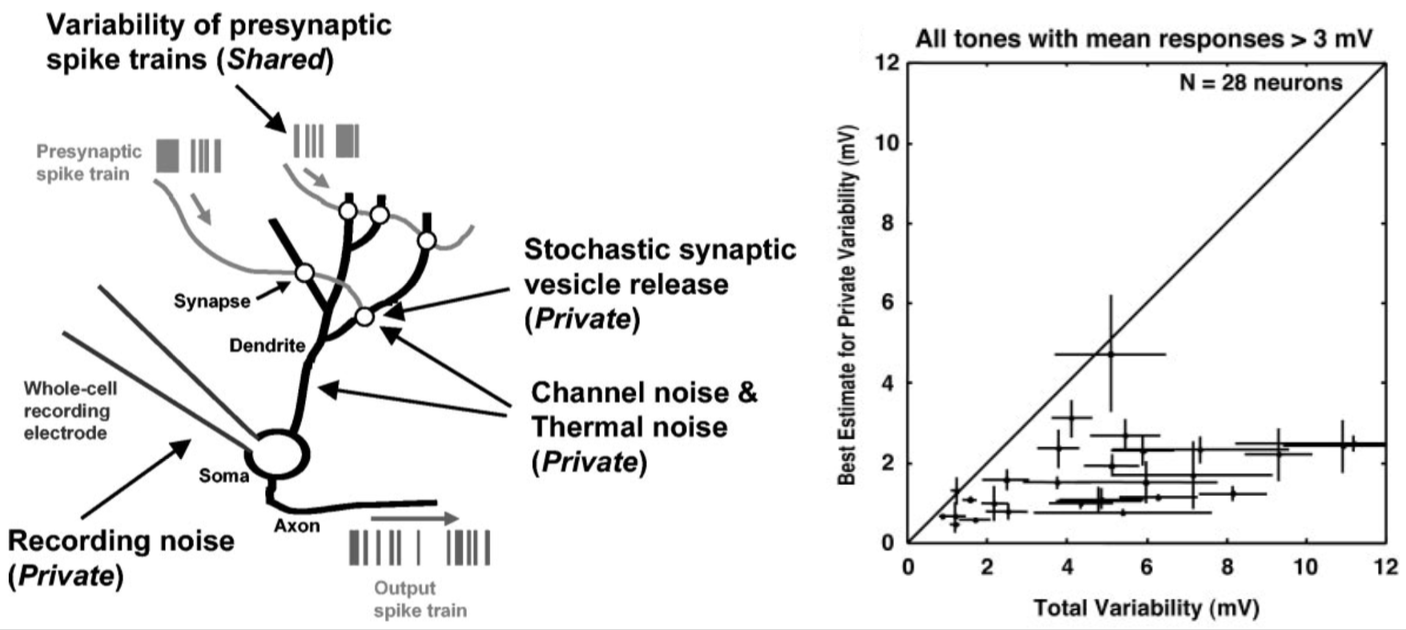
\includegraphics{img/figure1.png}}
		\caption{Shared and private variability.}
		\label{fig:private-shared}
	\end{figure}
	\newpage 
	
	\section{Methods}
	\subsection{Network Architecture}
	We consider the linear-nonlinear architecture depicted in Figure \ref{architecture}. The inputs to the network consist of a stimulus $s$ along with common (Gaussian) noise $\xi_C$. The $N$ neurons in the network take a linear combination of the inputs which is then corrupted by i.i.d. ``membrane potential'' Gaussian noise. Thus, the output of the linear stage for the $i$th neuron is 
	\begin{align}
		\ell_i &= v_i s + w_i \sigma_C \xi_C + \sigma_M\xi_{M,i},
	\end{align}
	where $\xi_{M,i}$ is the membrane potential noise. Both noise terms are scaled by positive constants $\sigma_C$ and $\sigma_M$ in order to make their variances explicit. The noisy linear combination is passed through a nonlinearity $g_i(\ell_i)$ whose output $r_i$ can be thought of as a firing rate. We consider the cases in which $\mathbf{r}$ alone serves as the network's output and when it acts as the mean for a Poisson firing process.
	
	Thus, the network-wide computation is given by
	\begin{align}
		\mathbf{r} &= \mathbf{g}(\mathbf{v} s + \mathbf{w} \sigma_C \xi_C +\sigma_M \boldsymbol{\xi}_M)
	\end{align}
	where vector notation denotes the weights, noises, and nonlinearities across the neuronal population. In this scheme the correlational structure of the network is dictated by the choice of weight vectors $\mathbf{v}$, $\mathbf{w}$ along with the array of nonlinearities $\mathbf{g}$. 
	\begin{figure}[ht]
		\centering
		\scalebox{1.0}{
			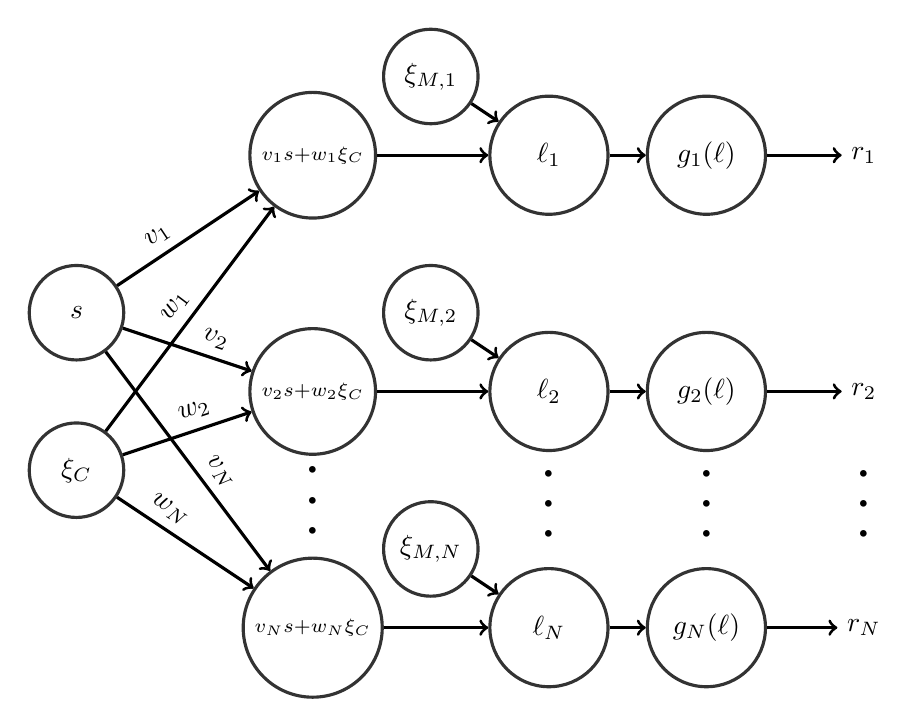
\begin{tikzpicture}
				\tikzstyle{main} = [circle, minimum size = 12mm, line width = 0.4mm, draw=black!80, node distance = 16mm]
				\tikzstyle{main2} = [circle, minimum size = 15mm, line width = 0.4mm, draw=black!80, node distance = 16mm]
				\node[main, fill = white!100] at (-2, 1.) (s) {$s$};
				\node[main, fill = white!100] at (-2, -1.) (common) {$\xi_C$};
				
				\node[main2] at (1.,3.0)  (l1) {${\scriptstyle v_1 s + w_1 \xi_C}$};
				\node[main2] at (1.,0.0)  (l2) {${\scriptstyle v_2 s + w_2 \xi_C}$};
				\node[main2] at (1,-3.0) (lN) {${\scriptstyle v_N s + w_N \xi_C}$};
				
				\node[main2] at (4.,3.0)  (ell1) {$\ell_1$};
				\node[main2] at (4.,0.0)  (ell2) {$\ell_2$};
				\node[main2] at (4,-3.0) (ellN) {$\ell_{N}$};
				
				\node[main2] at (6, 3.0) (nonlin1) {$g_1(\ell)$};
				\node[main2] at (6, 0.0) (nonlin2) {$g_2(\ell)$};
				\node[main2] at (6, -3.0) (nonlinN) {$g_N(\ell)$};
				
				\node at (8, 3.0) (r1) {$r_1$};
				\node at (8, 0.0) (r2) {$r_2$};
				\node at (8, -3.0) (rN) {$r_N$};
				
				\node[main] at (2.5, 4.0) (xi1) {$\xi_{M,1}$};
				\node[main] at (2.5, 1.0) (xi2) {$\xi_{M,2}$};
				\node[main] at (2.5, -2.0) (xiN) {$\xi_{M,N}$};
				
				\draw[->, line width = 0.4mm] (s) -- (l1) node[midway, above left, sloped] {$v_1$};
				\draw[->, line width = 0.4mm] (s) -- (l2) node[midway, above right, sloped] {$v_2$};
				\draw[->, line width = 0.4mm] (s) -- (lN) node[midway, above right, sloped] {$v_N$};
				
				\draw[->, line width = 0.4mm] (common) -- (l1) node[pos = 0.6, above left, sloped] {$w_1$};
				\draw[->, line width = 0.4mm] (common) -- (l2) node[pos = 0.8, above left, sloped] {$w_2$};
				\draw[->, line width = 0.4mm] (common) -- (lN) node[midway, above left, sloped] {$w_N$};
				
				\draw[->, line width = 0.4mm] (l1) -- (ell1);
				\draw[->, line width = 0.4mm] (l2) -- (ell2);
				\draw[->, line width = 0.4mm] (lN) -- (ellN);
				
				\draw[->, line width = 0.4mm] (xi1) -- (ell1);
				\draw[->, line width = 0.4mm] (xi2) -- (ell2);
				\draw[->, line width = 0.4mm] (xiN) -- (ellN);
				
				\draw[->, line width = 0.4mm] (ell1) -- (nonlin1);
				\draw[->, line width = 0.4mm] (ell2) -- (nonlin2);
				\draw[->, line width = 0.4mm] (ellN) -- (nonlinN);
				
				\draw[->, line width = 0.4mm] (nonlin1) -- (r1);
				\draw[->, line width = 0.4mm] (nonlin2) -- (r2);
				\draw[->, line width = 0.4mm] (nonlinN) -- (rN);
				
				\path (l2) -- (lN) node [black, font=\Huge, midway, sloped] {$\dots$};
				\path (ell2) -- (ellN) node [black, font=\Huge, midway, sloped] {$\dots$};
				\path (nonlin2) -- (nonlinN) node [black, font=\Huge, midway, sloped] {$\dots$};
				\path (r2) -- (rN) node [black, font=\Huge, midway, sloped] {$\dots$};	
			\end{tikzpicture}}
%		\scalebox{0.75}{
%		\begin{tikzpicture}
%			\tikzstyle{main} = [circle, minimum size = 12mm, line width = 0.4mm, draw=black!80, node distance = 16mm]
%			\tikzstyle{main2} = [circle, minimum size = 15mm, line width = 0.4mm, draw=black!80, node distance = 16mm]
%			\node[main, fill = white!100] at (-2, 2.) (s) {$s$};
%			\node[main, fill = white!100] at (-2, 0.) (inj) {$\xi_I$};
%			\node[main, fill = white!100] at (-2, -3.) (ink) {$\xi^I_k$};
%			
%			\node[main2] at (1.,3.0)  (c1) {${\scriptstyle v_1 s + w_1 \xi_I}$};
%			\node[main2] at (1.,0.0)  (c2) {${\scriptstyle v_2 s + w_2 \xi_I}$};
%			\node[main2] at (1,-3.0) (cN) {${\scriptstyle v_N s + w_N \xi_I}$};
%			
%			\node[main2] at (4.,3.0)  (lin1) {$\ell_1$};
%			\node[main2] at (4.,0.0)  (lin2) {$\ell_2$};
%			\node[main2] at (4,-3.0) (linN) {$\ell_{N}$};
%			
%			\node[main2] at (6, 3.0) (nonlin1) {$g_1(\ell)$};
%			\node[main2] at (6, 0.0) (nonlin2) {$g_2(\ell)$};
%			\node[main2] at (6, -3.0) (nonlinN) {$g_N(\ell)$};
%			
%			\node at (8, 3.0) (r1) {$r_1$};
%			\node at (8, 0.0) (r2) {$r_2$};
%			\node at (8, -3.0) (rN) {$r_N$};
%			
%			\node[main] at (2.5, 4.0) (xi1) {$\xi_1^M$};
%			\node[main] at (2.5, 1.0) (xi2) {$\xi_2^M$};
%			\node[main] at (2.5, -2.0) (xiN) {$\xi_N^M$};
%			
%			\draw[->, line width = 0.4mm] (s) -- (c1) node[midway, above left, sloped] {$v_1$};
%			\draw[->, line width = 0.4mm] (s) -- (c2) node[midway, above right, sloped] {$v_2$};
%			\draw[->, line width = 0.4mm] (s) -- (cN) node[midway, above right, sloped] {$v_N$};
%			
%			\draw[->, line width = 0.4mm] (inj) -- (c1) node[pos = 0.6, above left, sloped] {$w_1$};
%			\draw[->, line width = 0.4mm] (inj) -- (c2) node[pos = 0.8, above left, sloped] {$w_2$};
%			\draw[->, line width = 0.4mm] (inj) -- (cN) node[midway, above left, sloped] {$w_N$};
%			
%			\draw[->, line width = 0.4mm] (ink) -- (c1) node[pos = 0.6, above left, sloped] {$w_1$};
%			\draw[->, line width = 0.4mm] (ink) -- (c2) node[pos = 0.8, above left, sloped] {$w_2$};
%			\draw[->, line width = 0.4mm] (ink) -- (cN) node[midway, above left, sloped] {$w_N$};
%			\draw[->, line width = 0.4mm] (c1) -- (lin1);
%			\draw[->, line width = 0.4mm] (c2) -- (lin2);
%			\draw[->, line width = 0.4mm] (cN) -- (linN);
%			
%			\draw[->, line width = 0.4mm] (xi1) -- (lin1);
%			\draw[->, line width = 0.4mm] (xi2) -- (lin2);
%			\draw[->, line width = 0.4mm] (xiN) -- (linN);
%			
%			\draw[->, line width = 0.4mm] (lin1) -- (nonlin1);
%			\draw[->, line width = 0.4mm] (lin2) -- (nonlin2);
%			\draw[->, line width = 0.4mm] (linN) -- (nonlinN);
%			
%			\draw[->, line width = 0.4mm] (nonlin1) -- (r1);
%			\draw[->, line width = 0.4mm] (nonlin2) -- (r2);
%			\draw[->, line width = 0.4mm] (nonlinN) -- (rN);
%			
%			\path (inj) -- (ink) node [black, font=\Huge, midway, sloped] {$\dots$};
%			\path (c2) -- (cN) node [black, font=\Huge, midway, sloped] {$\dots$};
%			\path (lin2) -- (linN) node [black, font=\Huge, midway, sloped] {$\dots$};
%			\path (nonlin2) -- (nonlinN) node [black, font=\Huge, midway, sloped] {$\dots$};
%			\path (r2) -- (rN) node [black, font=\Huge, midway, sloped] {$\dots$};	
%			\end{tikzpicture}
%		}
		\caption{Linear-Nonlinear Network Architecture. The network takes as its inputs a stimulus $s$ and common noise $\xi_C$. A linear combination of these quantities is corrupted by individual membrane potential noise $\xi_{M,i}$. The output of this linear stage is then passed through a nonlinearity $g_i(\ell)$.}
		\label{architecture}
	\end{figure}
	
	\subsection{Measures of Coding Strength}
	In order to assess the fidelity of the population code represented by $\boldsymbol{\ell}$ or $\mathbf{r}$, we turn to the Fisher information and the Shannon mutual information. The former has largely been utilized in the context of sensory decoding and correlated variability \cite{2016kohn} while the latter has been well studied in the context of efficient coding. The Fisher information sets a limit by which the readout of a population code can determine the input. Formally, it sets a lower bound to the variance of an estimator. Often, the Fisher information is intractable to calculate analytically; a suitable lower bound is the linear Fisher information:
	\begin{align}
		I_F(s) &= \mathbf{f}'(s)^T \boldsymbol{\Sigma}^{-1}(s) \mathbf{f}(s)
	\end{align}
	whose corresponding estimator is the locally optimal linear estimator. 
	\subsection{Structured Weights}
	To obtain analytic expressions for these quantities, we first consider the case of ``structured weights'' taking on the form
	\begin{align}
		c \times \left(\underbrace{1 \cdots 1}_{N/k \text{ times}}  \ \underbrace{2 \cdots 2}_{N/k \text{ times}} \ \cdots \ \underbrace{k \cdots k}_{N/k \text{ times}}   \right)^T.
	\end{align}
	Specifically, the structured weight vectors are parameterized by an integer $k$ which divides the $N$ weights into $k$ homogeneous groups. The weights across the groups span the positive integers up to $k$, and we allow for a final scaling factor $c$. 
	
	Importantly,  larger $k$ will only increase the weights in the vector. Thus, in the above scheme, increased ``diversity'' can only be achieved through an increase through the parameter $k$, which will invariably result in an amplification of the signal to which the weight vector is applied. In the case that $k$ does not evenly divide $N$, the last group is repeated $N\text{mod }k$ times.
	
	\subsection{Unstructured Weights}
	
	While the structured weights provide us analytic results, they possess an unrealistic distribution of synaptic weighting. Thus, we turn to the case of ``unstructured weights,'' in which the synaptic weights are drawn from some parameterized probability distribution:
	\begin{align}
		\mathbf{v} \sim p(\mathbf{v}; \theta_{\mathbf{v}}); \ \mathbf{w} \sim p(\mathbf{w}; \theta_{\mathbf{w}}).
	\end{align}
	Thus, we  calculate both information theoretic quantities over many random draws from these distributions. We then observe how the quantities behave as some subset of the parameters $\theta$ are varied. In particular, we will focus on the lognormal distribution, which has been observed to describe the distribution of synaptic weights well in slice electrophysiology \textcolor{red}{[citation]}. Specifically, we examine 
	\begin{align}
		\mathbf{w}\sim \text{Lognormal}(\mu - \Delta, \sigma)
	\end{align}
	where $\Delta$ sets a lower bound for the weights. Here, increased ``diversity'' in the sense of the structured weights is achieved by increasing $\mu$, which increases the mean, median, and mode of the lognormal distribution. This is in contrast with increasing $\sigma$, which will decrease the mode of the distribution.
	\newpage
	
	\section{Results}
	We consider the network's coding ability after both the linear stage $(\boldsymbol{\ell})$ and the nonlinear stage $(\mathbf{r})$. The linear stage can be considered the output of the network assuming the functions $\mathbf{g}$ are simply the identity. Furthermore, the qualitative conclusions we obtain from the linear stage should be  We consider both the structured and unstructured cases.
	\subsection{Linear Stage}
	The Fisher information in the linear representation is calculated in Appendix \ref{app:fisher-linear} as 
	\begin{align}
		I_F(s) &= \frac{1}{\sigma_M^2}\frac{\left(\sigma_M^2/\sigma_C^2\right) |\mathbf{v}|^2 +  \left(|\mathbf{v}|^2|\mathbf{w}|^2 - (\mathbf{v}\cdot\mathbf{w})^2\right)}{(\sigma_M^2/\sigma_C^2)+ |\mathbf{w}|^2}. \label{eqn:fisher-linear}
	\end{align}
	while the mutual information is calculated in Appendix \ref{mutual-linear} as
	\begin{align}
		I[s, \boldsymbol{\ell}] &= \frac{1}{2} \log \left(1 + \frac{\sigma_S^2}{\sigma_M^2} |\mathbf{v}|^2 - \frac{\sigma_S^2}{\sigma_M^2} \frac{(\mathbf{v}\cdot\mathbf{w})^2}{(\sigma_M^2/\sigma_C^2) + |\mathbf{w}|^2}\right). \label{eqn:mutual-linear}
	\end{align}
	In the case of mutual information, we have assumed the stimulus prior is Gaussian with zero mean and standard deviation $\sigma_S$. For structured weights, equations \ref{eqn:fisher-linear} and \ref{eqn:mutual-linear} can be explored by varying the choice of $k$ for both $\mathbf{v}$ and $\mathbf{w}$ (call them $k_{\mathbf{v}}$ and $k_{\mathbf{w}}$, respectively).
	
	It is simplest to examine these quantities with $k_{\mathbf{v}}=1$ while allowing $k_{\mathbf{w}}$ to vary, as amplifying and diversifying $\mathbf{v}$ will increase coding ability (which our results corroborate) \cite{Ecker2011}. On the other hand, while increasing $k_{\mathbf{w}}$ will boost the overall noise added into the neural population, it also changes the direction that the noise is projected into the higher-dimensional neural space. Thus, while we might expect that more noise in the system would hinder coding, the direction to which the noise is projected is important. 
	
	We first consider how the Fisher information and mutual information are impacted by the choice of $k_{\mathbf{w}}$. In the structured regime, we have 
	\begin{align}
		|\mathbf{v}|^2 &= N \\
		\mathbf{v}\cdot\mathbf{w} &= \frac{N}{k} \sum_{i=1}^k i = \frac{N(k+1)}{2} \\
		|\mathbf{w}|^2 &= \frac{N}{k}\sum_{i=1}^k i^2 = \frac{N(k+1)(2k+1)}{6},
	\end{align}
	which allows us to write equations \ref{eqn:fisher-linear} and \ref{eqn:mutual-linear} as 
	\begin{align}
		I_F(s) = I_F &= \frac{N}{2\sigma_M^2} \frac{12 (\sigma_M^2/\sigma_C^2) + N  (k^2-1)}{6(\sigma_M^2/\sigma_C^2)+ N(2k^2+3k+1)} \\
		I[s, \boldsymbol{\ell}] &= \frac{1}{2} \log\left[1 + \frac{\sigma_S^2}{\sigma_M^2} N - \frac{\sigma_S^2}{\sigma_M^2}\frac{3N^2(k+1)^2}{2\sigma_M^2 \left(N\sigma_C^2(k+1)(2k+1) + 6 \sigma_M^2\right)}\right]
	\end{align}
	The structured regime analytically reveals the asymptotic behavior of the information quantities. Both quantities saturate as a function of $N$  only in the case of $k_{\mathbf{w}}=1$ (Figure \ref{fig:struct-linear}A, B); otherwise, they increase without bound. As expected, increasing the population of the system also enhances coding fidelity. Furthermore, both quantities are monotonically increasing functions of $k_{\mathbf{w}}$ (Figure \ref{fig:struct-linear}C, D), implying that encoding and decoding are enhanced despite the fact that the common noise is magnified for larger $k_{\mathbf{w}}$. Our analytic results ensure linear and logarithmic growth for the Fisher and mutual information, respectively, as one might expect in the case of Gaussian noise \cite{Brunel1998}. These qualitative results hold for any choice of $(\sigma_S, \sigma_M, \sigma_C)$.
	
	In the case of $k_{\mathbf{w}}=1$, the signal and noise are aligned perfectly in the neural representation, implying that the common noise becomes equivalent in form to shared input noise. In this scenario, we observe the saturation of both Fisher and mutual informations as a function of the neural population. Such saturation implies the existence of differential correlations, consistent with the observation that information-limiting correlations occur under the presence of shared input noise \cite{Moreno-Bote2014}.
	
	\begin{figure}[t]
		\centering
		\scalebox{0.35}{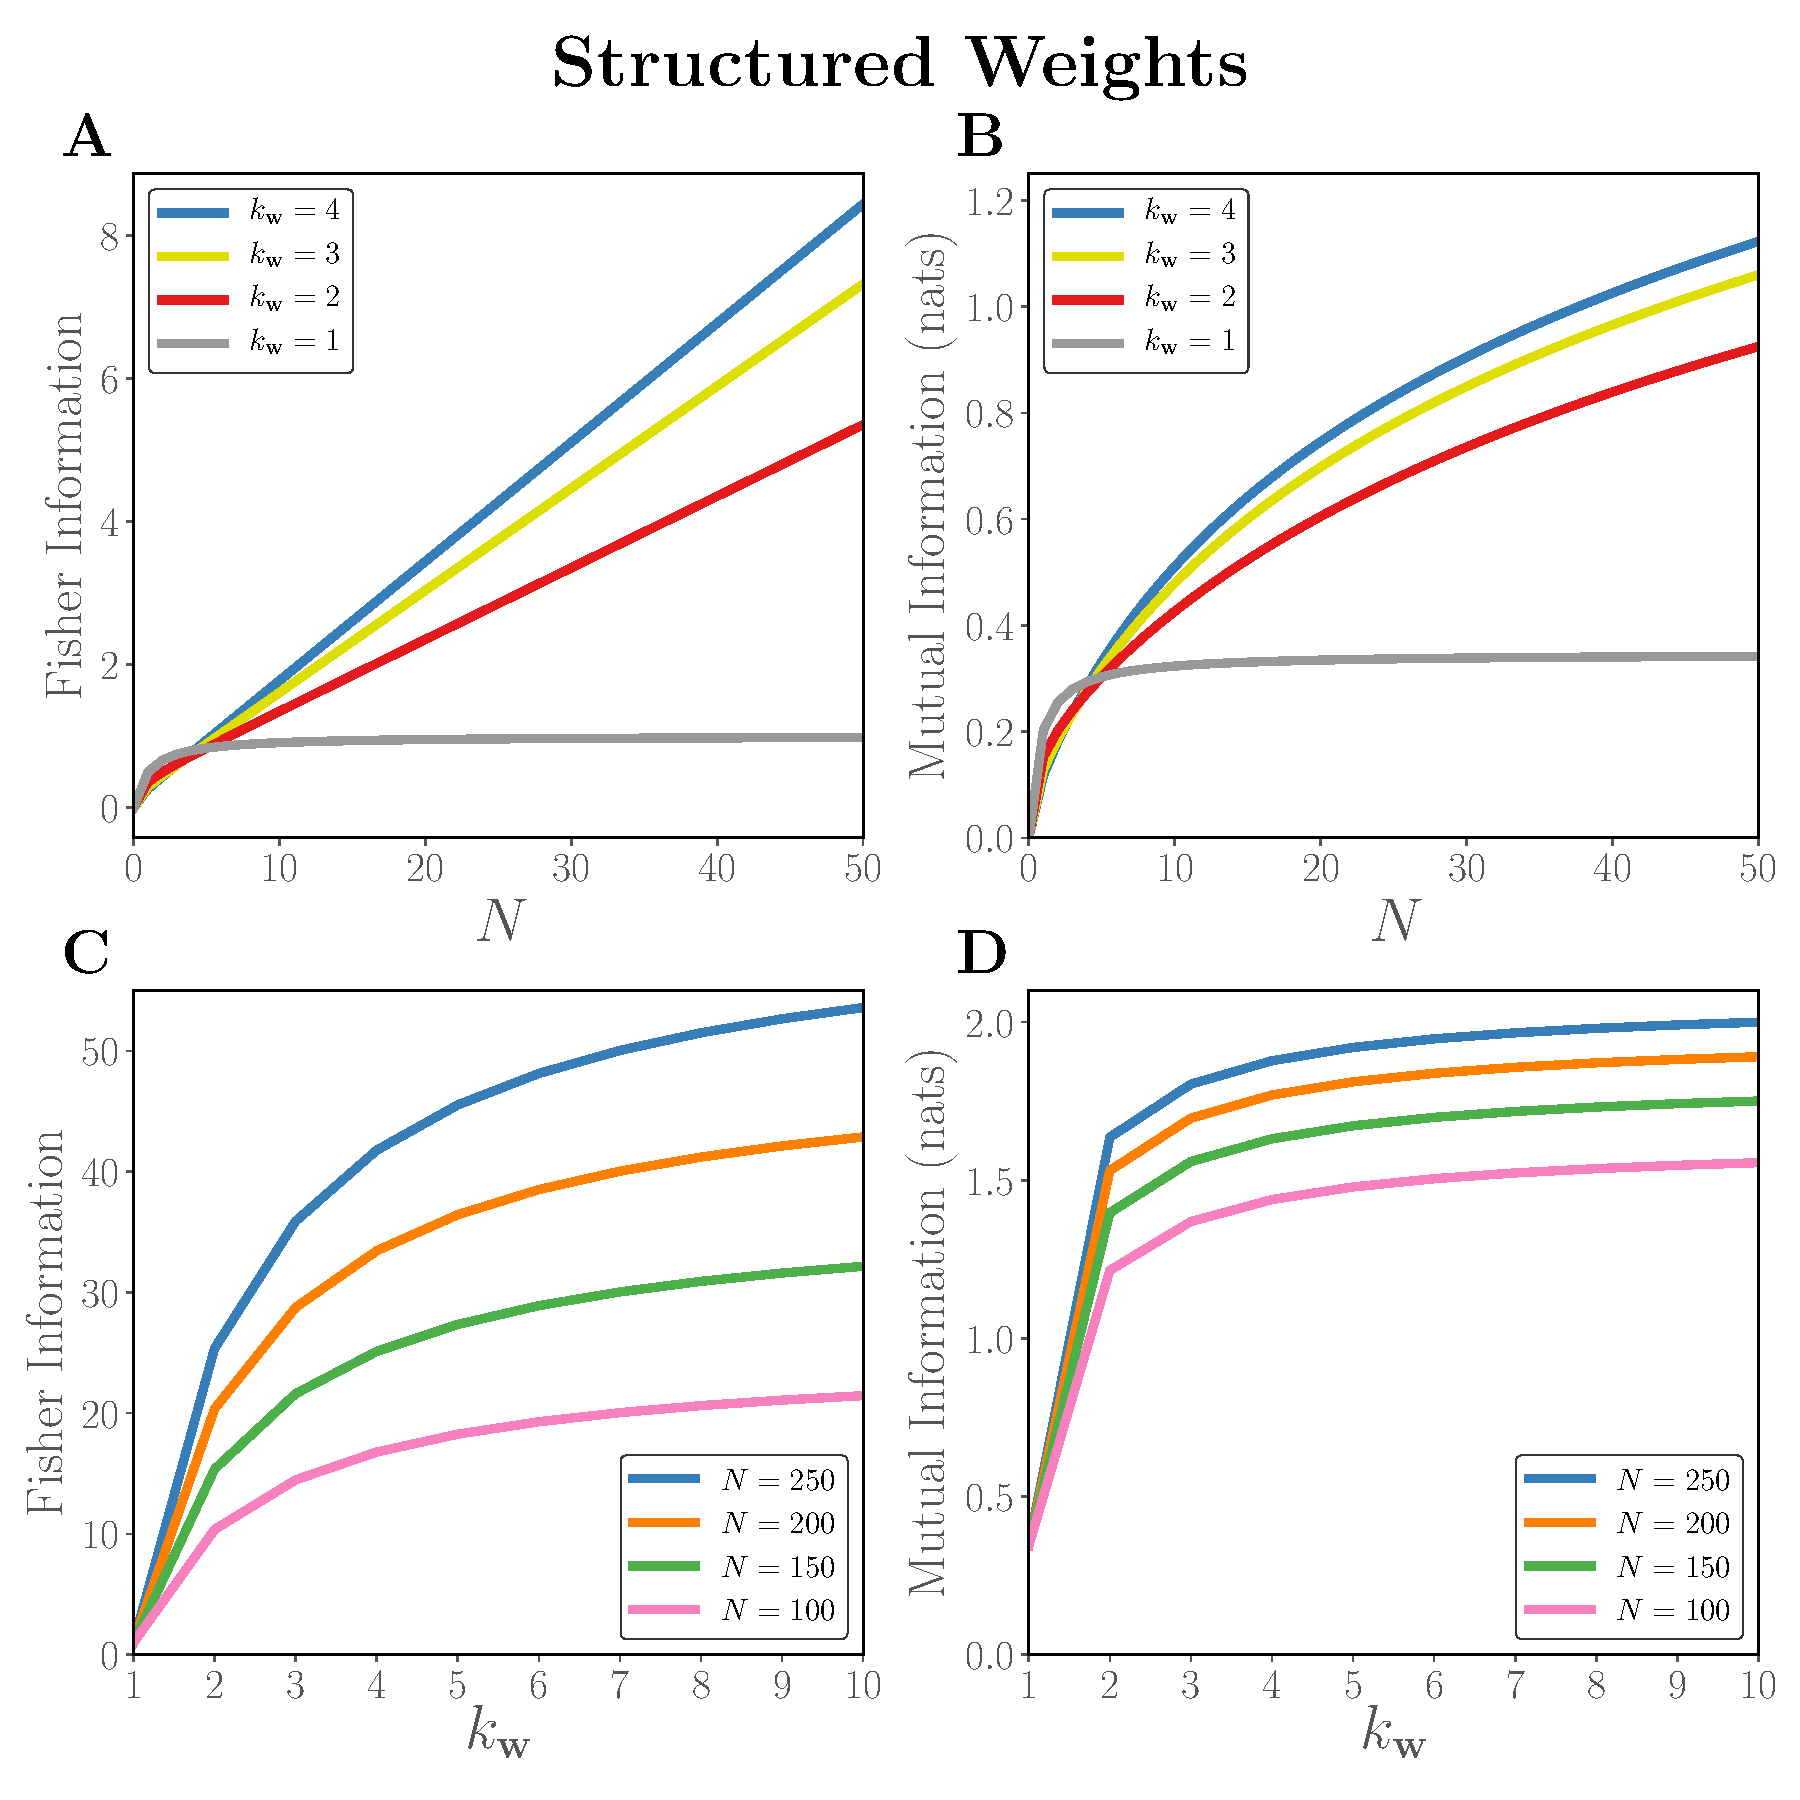
\includegraphics{img/figure2-part1.pdf}}
		\scalebox{0.35}{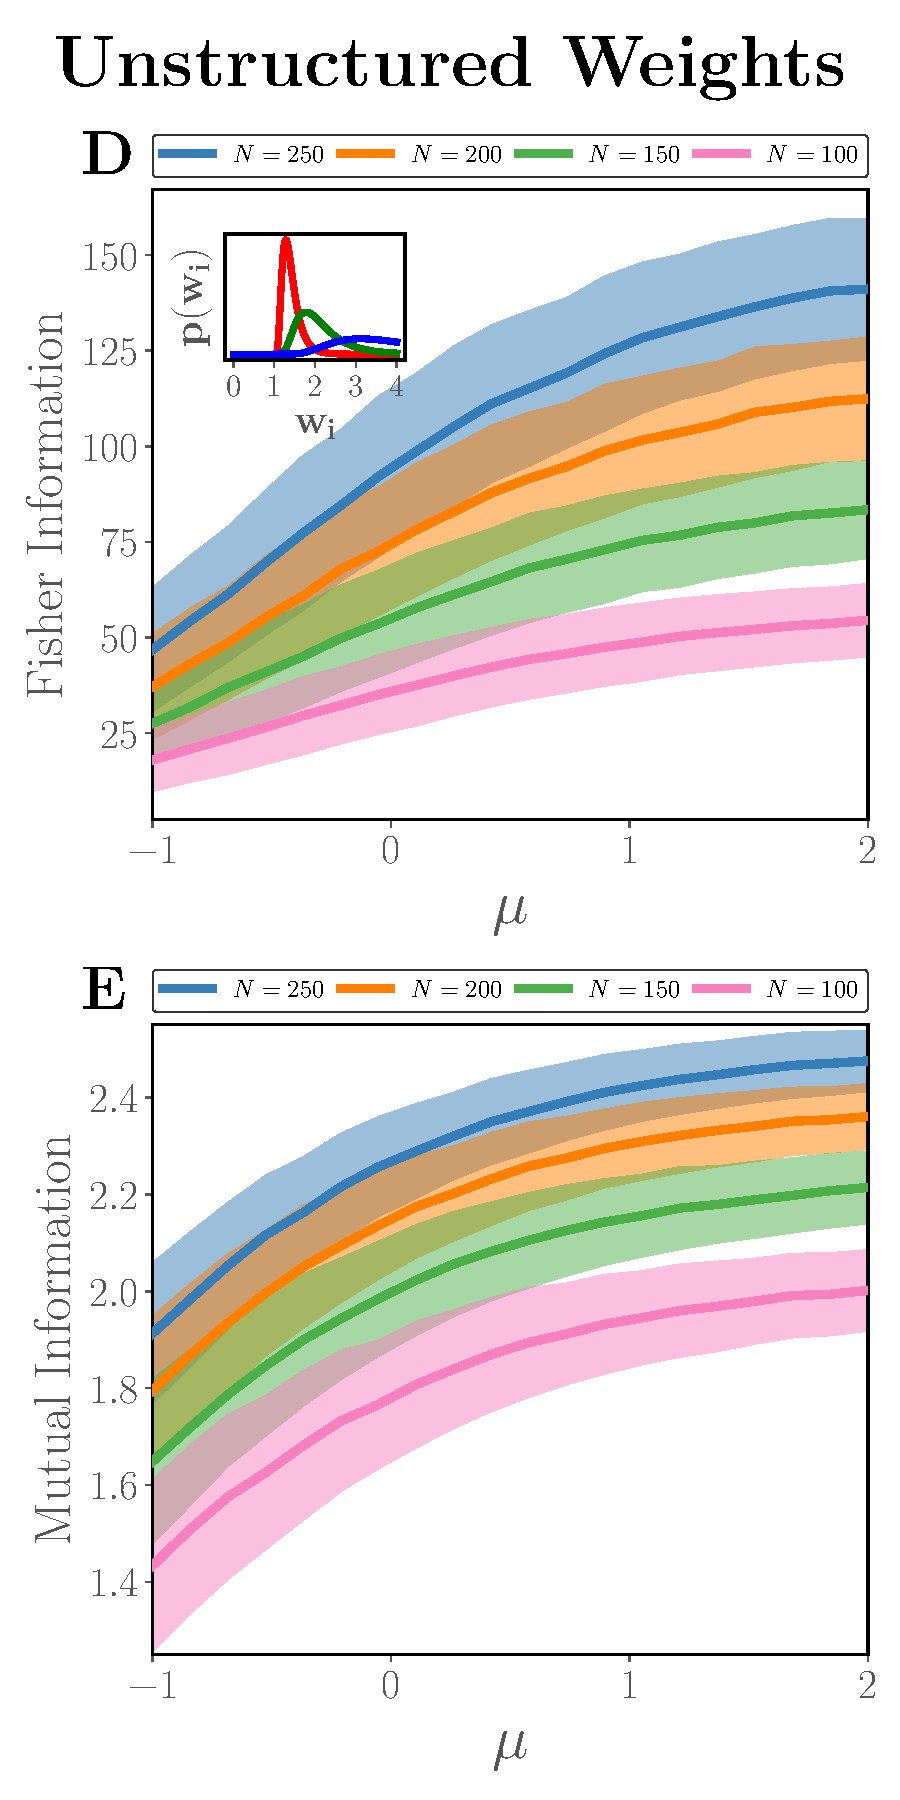
\includegraphics{img/figure2-part2.pdf}}
		\caption{The performance of the Fisher and mutual informations after the linear stage of the network. Here, we take $\sigma_M = \sigma_C=1$. Note that the Fisher information is independent of $s$. \textbf{(A)}, \textbf{(B)} Structured weights. Both informations saturate as a function of the number of neurons in the case of uniform noise weights ($k_{\mathbf{w}}=1$). Once $k_{\mathbf{w}}$ is increased, the informations are unbounded with respect to population size. \textbf{(C)}, \textbf{(D)} Same aforementioned network, but plotted with respect to heterogeneity for various network sizes. Increasing heterogeneity improves coding performance. \textbf{(E)}, \textbf{(F)} Unstructured weights calculated over 3000 draws from lognormal distributions. Inset shows the distribution of weights for various choices of $\mu$. Increasing $\mu$ shifts the distribution to the right, increasing heterogeneity. Means are indicated by solid lines while shaded region indicates one standard deviation.}\label{fig:struct-linear}
	\end{figure}
	
	While the structured weights provide us analytic results, they possess an unrealistic distribution of synaptic weighting. Thus, we turn to the case of ``unstructured weights,'' in which the synaptic weights are drawn from a shifted lognormal distribution \textcolor{red}{[citations]}. In this case, we calculate both information theoretic quantities over many random draws according to $w_i \sim \text{Lognormal}(\mu - \Delta, \sigma^2)$. We are primarily concerned with varying $\mu$, as increasing this quantity uniformly increases the mean, median, and mode of the lognormal distribution (Figure  \ref{fig:struct-linear}E, inset). Our numerical analysis demonstrates that increasing $\mu$ (akin to increasing $k_{\mathbf{w}}$) will increase the average Fisher information and average mutual information for multiple network sizes (Figure \ref{fig:struct-linear}E, F: bold lines). Thus, we once again observe that larger heterogeneity affords the network improved coding performance despite the overall increase in noise.

\begin{figure}[t]
	\centering
	\scalebox{0.27}{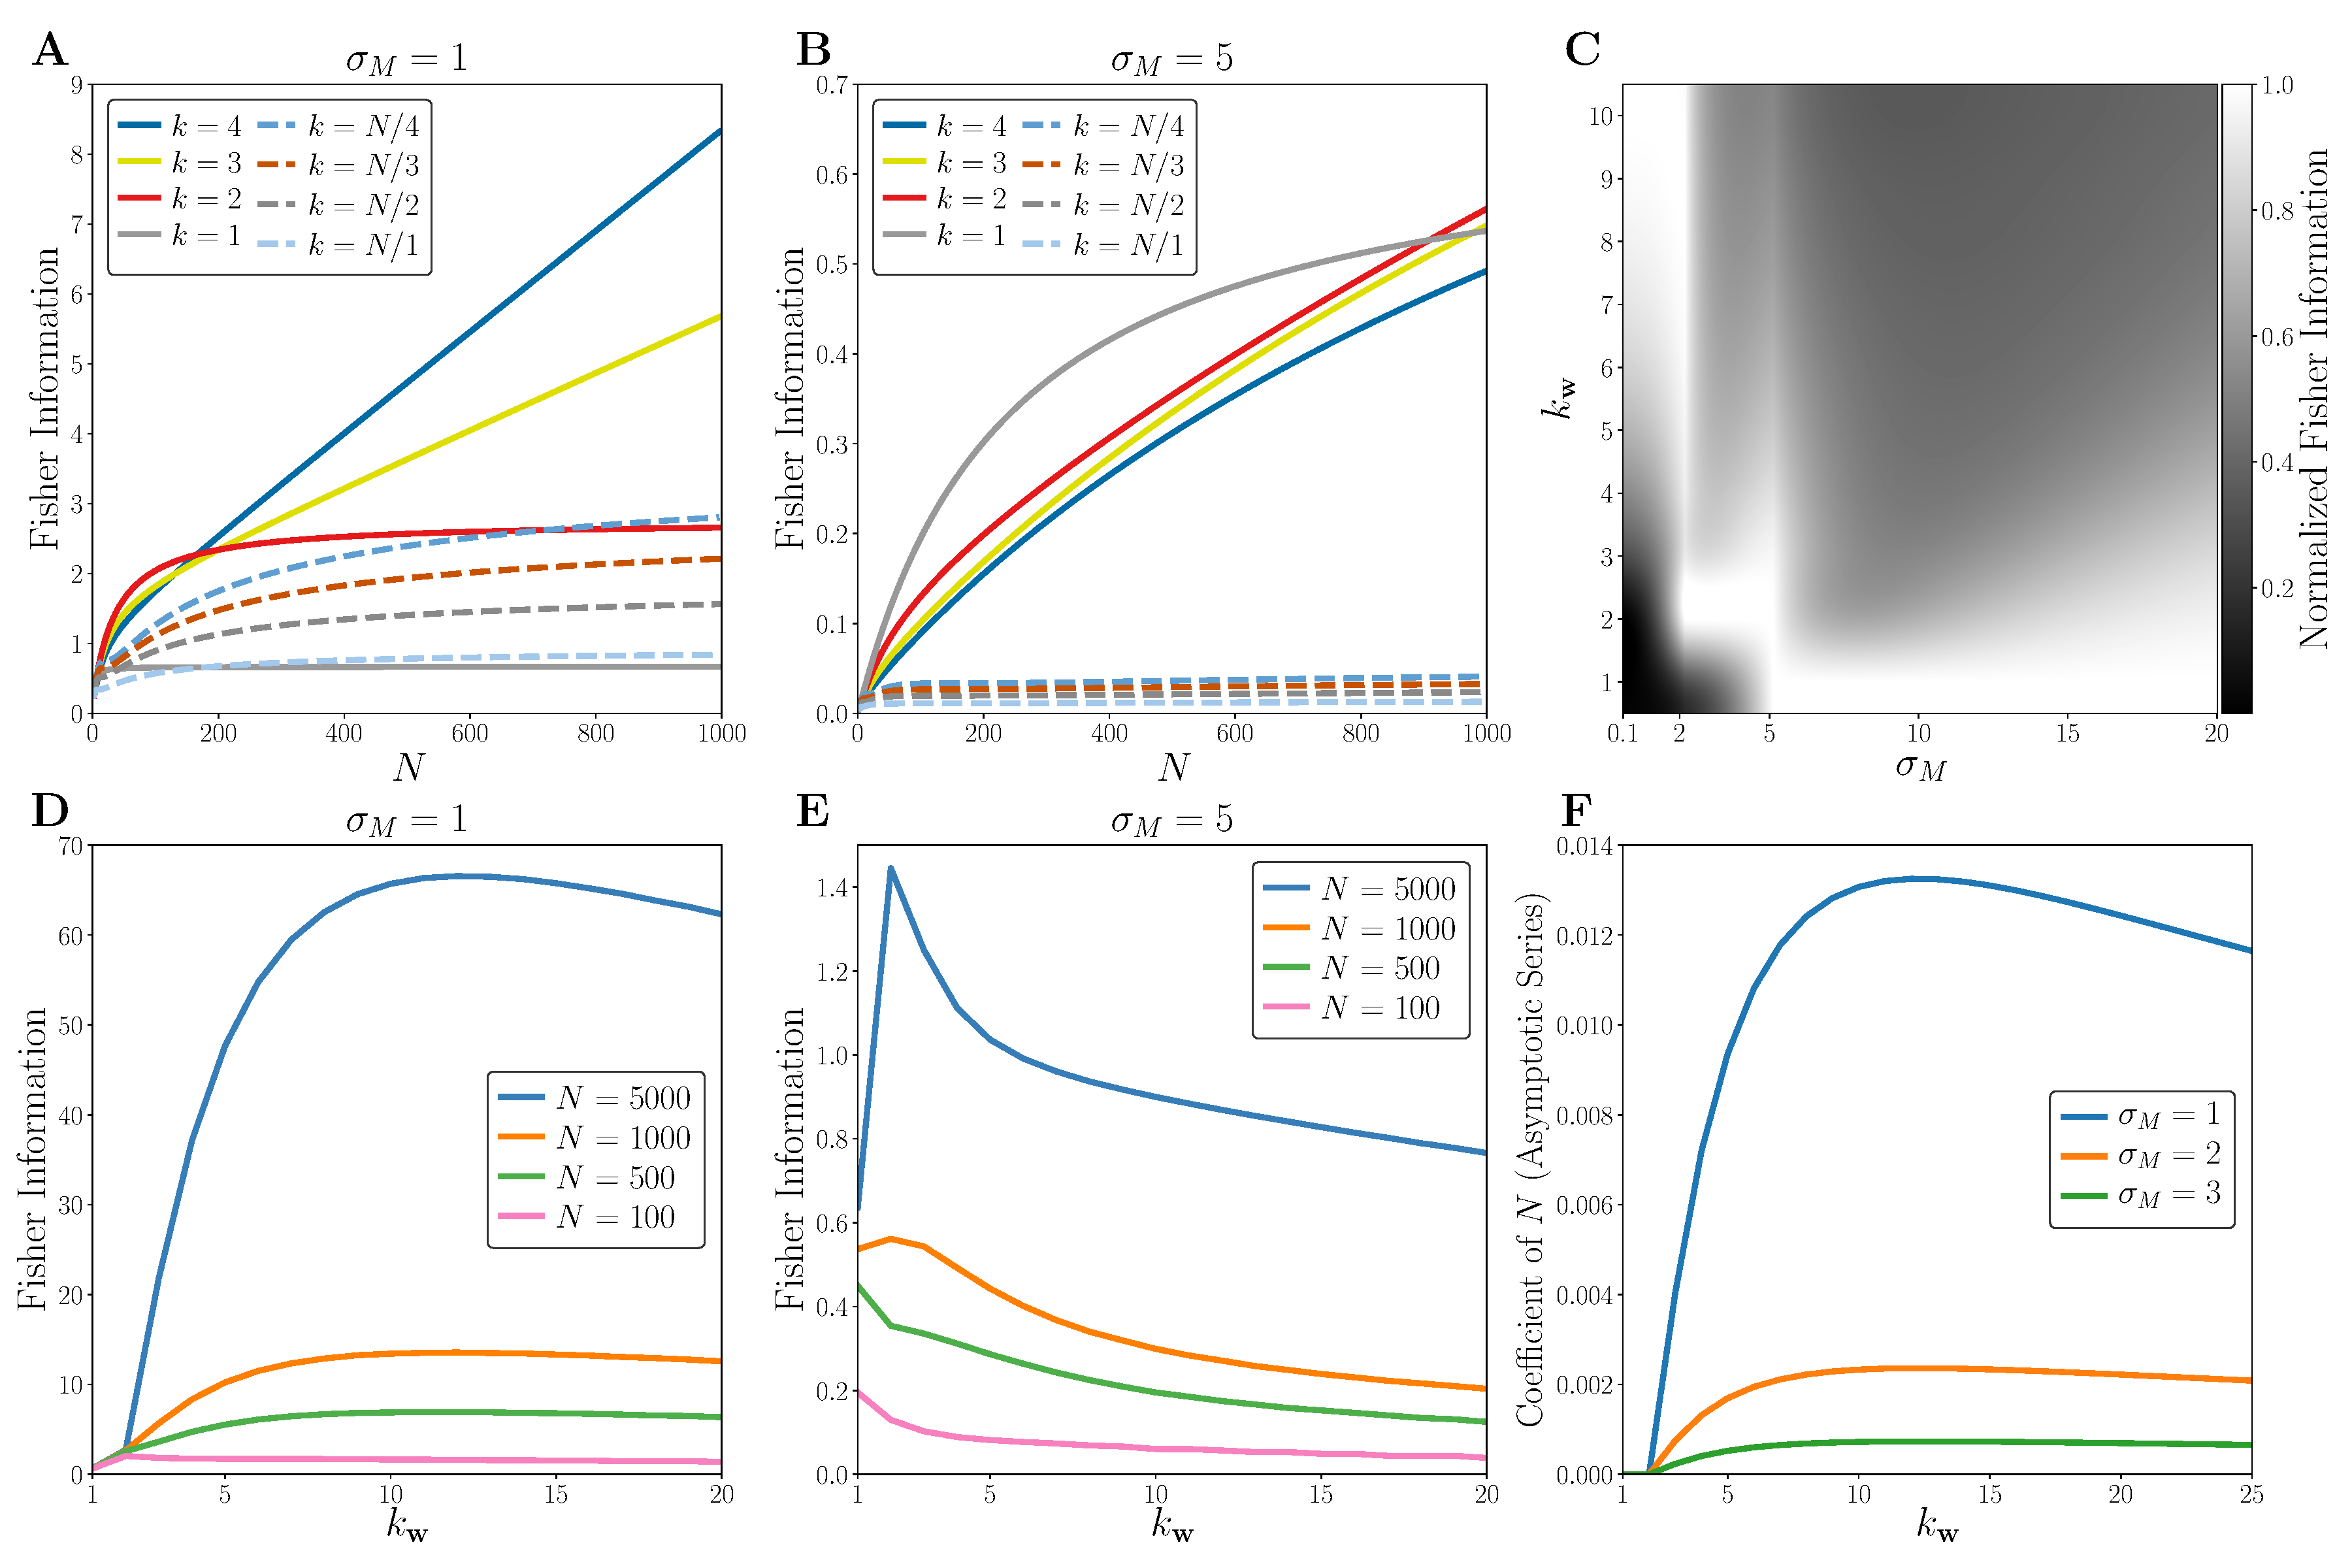
\includegraphics{img/figure3.pdf}}
	\caption{Fisher information in the network after a squared nonlinearity for structured weights. \textbf{(A)} When the membrane noise variance is equal to the common noise variance, we observe saturating behavior for $k=1$ and $k=2$. Increasing $k$ results in unbounded growth. At the extreme end of heterogeneity, where $k$ scales as $N$, the Fisher information saturates. \textbf{(B)} This qualitative behavior depends on the choice of $\sigma_M$. Increasing the membrane noise variance requires a much larger neural population to see the benefits of larger heterogeneity. \textbf{(C)} The Fisher information is normalized across all values of $\sigma_M/\sigma_C$ for a choice of $k$. The behavior of the Fisher information exhibits several phase transitions. This qualitative behavior may change as $N$ is increased.}
	\label{fig:fisher-quadratic}
\end{figure}
	
	
	\subsection{Nonlinear Stage}
	We next consider the performance of the network after a quadratic nonlinearity $g_i(x) = x^2$ for all neurons $i$. In this case, both the Fisher information and mutual information are analytically intractable. Thus, we will instead turn to the linear Fisher information is feasible, which is feasible. In addition, we will approximate the mutual information numerically. it is calculated in Appendix \ref{app:fisher-quadratic}. Its analytic form is too complicated to be restated here, but we can examine its behavior in both the structured and unstructured cases.
	
	\subsubsection{Structured Weights}
	Let us turn to the structured weights with $k_{\mathbf{v}}=1$ and varying $k_{\mathbf{w}}$, as before. In this case, the qualitative behavior of the Fisher information is dependent on magnitude of the shared ($\sigma_C^2$) and private ($\sigma_M^2$) variances. For example, consider $\sigma_M = \sigma_C=1$ (Figure \ref{fig:fisher-quadratic}A): here, we see that the Fisher information saturates for both $k_{\mathbf{w}}=1$ and $k_{\mathbf{w}}=2$, but increases without bound for larger $k_{\mathbf{w}}$. We can also consider the other extreme, where $k_{\mathbf{w}}\sim O(N)$; in this case the Fisher information drastically decreases and  appears to saturate (Figure \ref{fig:fisher-quadratic}A, dashed lines).
	
	Increasing the private variability results in qualitatively different finite network behavior ($\sigma_M=5$, Figure \ref{fig:fisher-quadratic}B). At $N=1000$, we see that $k_{\mathbf{w}}=1$ and $k_{\mathbf{w}}=2$ exhibit much better performance relative to larger values of $k_{\mathbf{w}}$. Meanwhile, for $k_{\mathbf{w}} \sim O(N)$, the Fisher information quickly saturates. We note that the increase in private variability has decreased \textit{all} Fisher informations compared to $\sigma_M=1$ (compare the scales of Figure \ref{fig:fisher-quadratic}A, B). Furthermore, it is important to point out that Figure \ref{fig:fisher-quadratic} only highlights finite network behavior; indeed, as we will see, the asymptotic behavior is consistent no matter the choice of $\sigma_M$.
	
	The introduction of the squared nonlinearity produces qualitatively different behavior at the finite network level: in contrast with Figure \ref{fig:struct-linear}, increased heterogeneity does not automatically imply improved decoding. Indeed, there is a regime in which increased heterogeneity improves Fisher information, beyond which we see a reduction in decoding performance. If the private variability increases, this regime shrinks or becomes nonexistent, depending on the network size (Figure \ref{fig:fisher-quadratic}E). Furthermore, entering this regime for higher private variability requires smaller $k_{\mathbf{w}}$. 
	
	The results shown in Figure \ref{fig:fisher-quadratic}A, B imply that there is an interesting relationship between the network's decoding ability, its private variability, and its synaptic weight heterogeneity $k_{\mathbf{w}}$. To explore this further, we examined the behavior of the Fisher information at a finite network size ($N=1000$) as a function of both $\sigma_M$ and $k_{\mathbf{w}}$ (Figure \ref{fig:fisher-quadratic}C).  To account for the fact that an increase in private variability will decrease the Fisher information, we plot the \textit{normalized} Fisher information: for a given choice of $\sigma_M$, each Fisher information is divided by the maximum across a range of $k_{\mathbf{w}}$. Thus, Figure \ref{fig:fisher-quadratic}C allows us to examine what level of synaptic weight heterogeneity maximizes the Fisher information, given a private variability $\sigma_M$.
	
	Figure \ref{fig:fisher-quadratic} highlights several interesting regimes. When the private variability is small, the network benefits from larger weight heterogeneity. But as it is increased, the . When the private variability is large, we are better off having less heterogeneous weights, despite the threat of differential correlations: 
	
	Lastly, we validated the asymptotic behavior of the Fisher information as a function of the private noise by examining the coefficient of $N$ in its asymptotic series (Figure \ref{fig:fisher-quadratic}F). For $k_{\mathbf{v}}=1,2$, the coefficient is zero for any choice of $\sigma_M$, implying that the Fisher information always saturates. Increasing the heterogeneity allows the network to escape the differential correlations and achieve linear asymptotic growth. But if $k_{\mathbf{w}}$ becomes too large, the linear asymptotic growth begins to decrease. When $k_{\mathbf{w}}\sim O(N)$, the asymptotic series is always sublinear (not shown in Figure \ref{fig:fisher-quadratic}F).
	
	\begin{figure}[t]
		\centering
		\scalebox{0.27}{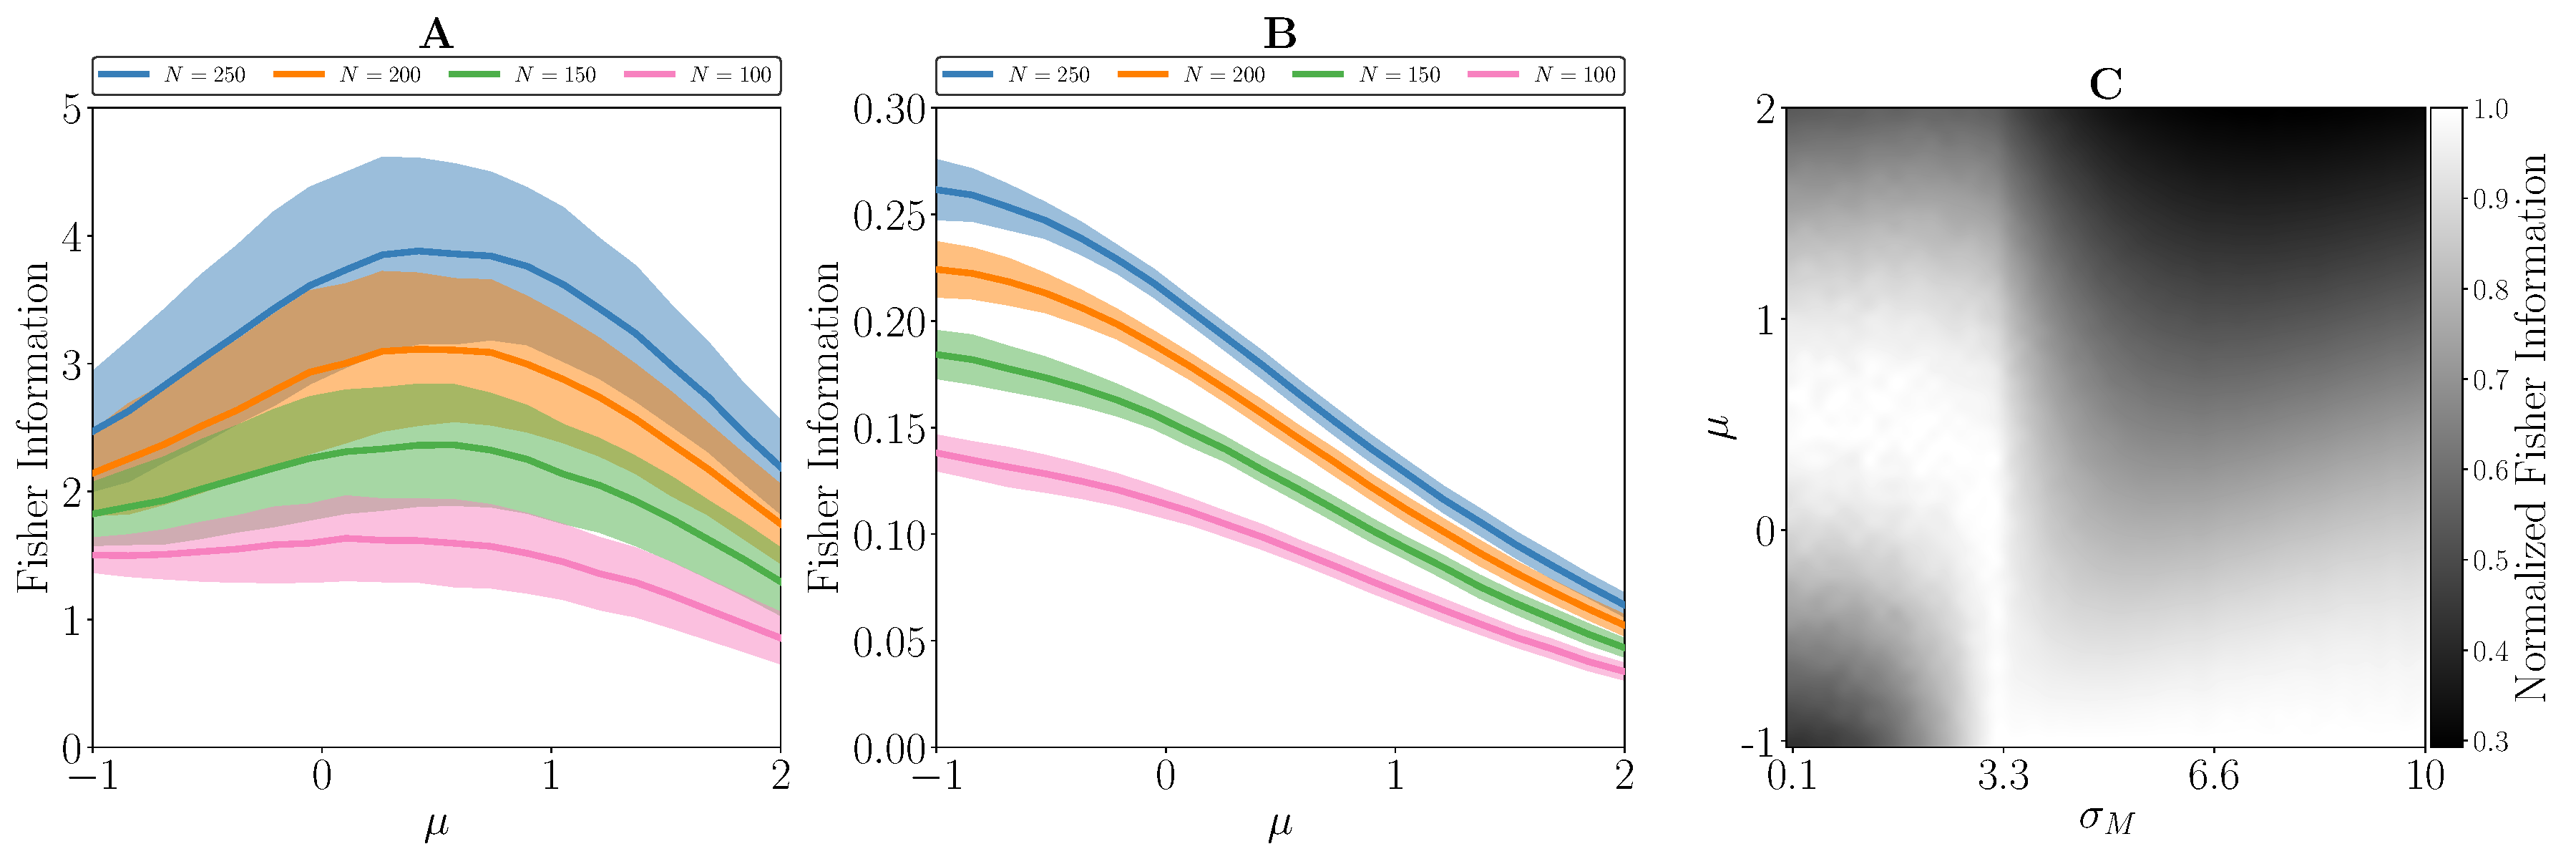
\includegraphics{img/figure4.pdf}}
		\caption{The behavior of the linear Fisher information for unstructured weights under the presence of a quadratic linearity. \textbf{(A)} } 
	\end{figure}
	\subsubsection{Unstructured Weights}
	We reproduced the above analysis with the unstructured weights, once again taking 3000 random draws from a shifted lognormal distribution. 
	
	\subsubsection{Mutual Information}
	Lastly, we examine the mutual information. For a quadratic nonlinearity, the mutual information is also analytically intractable. Thus, we use an 
	\subsection{The benefits of increased heterogeneity}
	Why are we afforded improved encoding and decoding as the common noise is amplified for certain neurons in the network? An increase in heterogeneity, as we have defined it, ensures that the common noise is magnified in the network. At the same time, however, the structure of the correlated variability induced by the common noise changes with increased heterogeneity. 
	
	At the linear stage, the answer appears to be clear: an increase in heterogeneity
	
	The network effective

	\begin{figure}[b]
		\centering
		\scalebox{0.27}{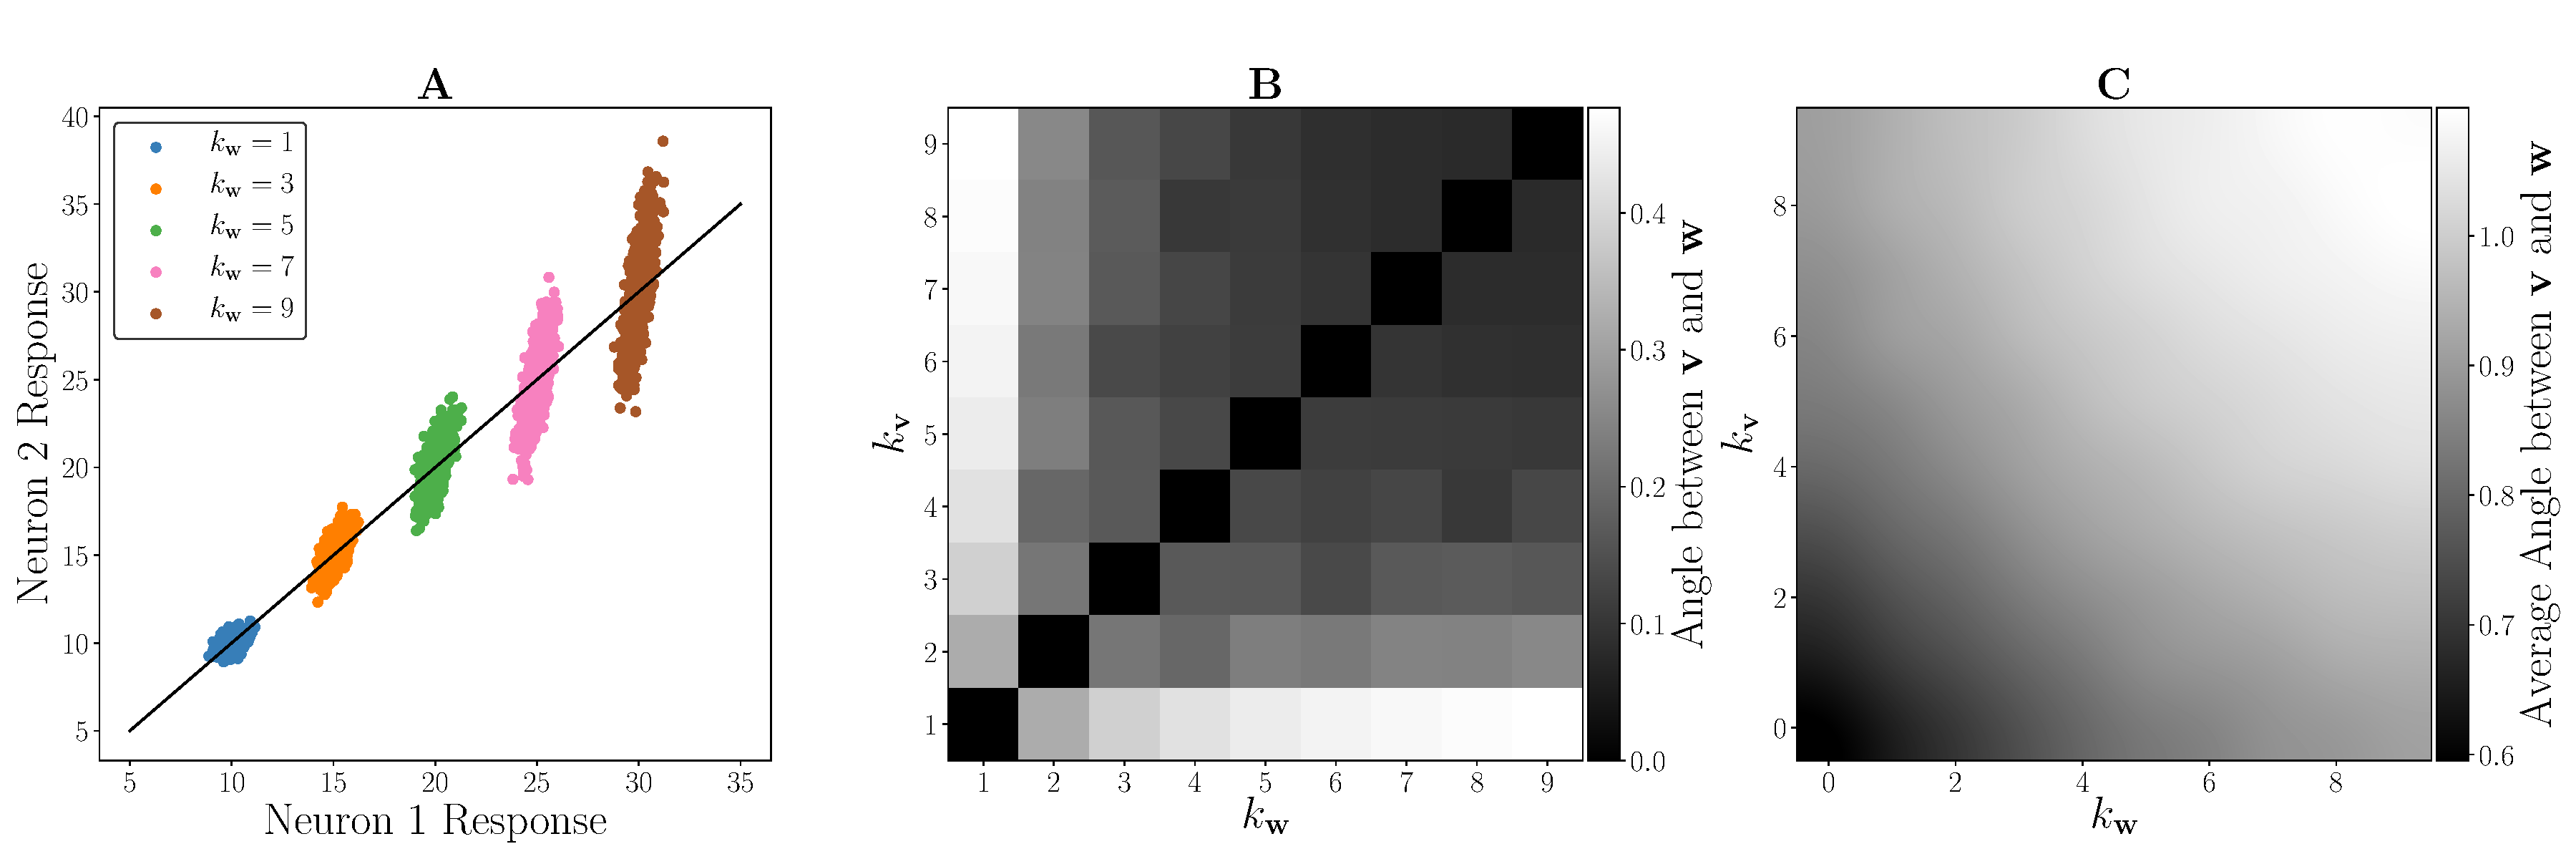
\includegraphics{img/figure5.pdf}}
		\caption{} 
	\end{figure}	
	\newpage
	\section{Discussion}
	

	\newpage
	%%% BIBLIOGRAPHY %%%
	\printbibliography

	\newpage
	
	\appendix
	\section{Calculation of  Fisher Information, Linear Stage}\label{app:fisher-linear}
	All variability after the linear stage is Gaussian; thus, the Fisher information can be expressed in the form \cite{1999abbott_dayan, 1993kay}:
	\begin{align}
		I_{F}(s) &= \mathbf{f}'(s)^T \boldsymbol{\Sigma}^{-1} (s) \mathbf{f}'(s) + \frac{1}{2}\Tr\left[\boldsymbol{\Sigma}'(s) \boldsymbol{\Sigma}^{-1}(s)\boldsymbol{\Sigma}'(s) \boldsymbol{\Sigma}^{-1}(s)\right]. \label{IF-gaussian}
	\end{align}
	Our immediate goal is to calculate $\mathbf{f}(s)$, the average response of the linear stage, and $\boldsymbol{\Sigma}$, the covariance between the responses. The output of the $i$th neuron after the linear stage is
	\begin{align}
		\ell_i &= v_i s + w_i \sigma_C \xi_C + \sigma_M\xi_{M,i},
	\end{align}
	so that the average response as a function of $s$ is
	\begin{align}
		f_i(s) &= \langle \ell_i \rangle = v_i s.
	\end{align}
	Thus,
	\begin{align}
		\mathbf{f}(s) = \mathbf{v}s \Rightarrow \mathbf{f}'(s) = \mathbf{v}.
	\end{align}
	
	Meanwhile,
	\begin{align}
		\langle \ell_i \ell_j \rangle &= \langle (v_i s + w_i \sigma_C\xi_C + \sigma_M\xi_{M,i}) (v_j s + w_j \sigma_C\xi_C + \sigma_M\xi_{M,j})\rangle \\
		&= v_i v_j s^2 + w_i w_j \sigma_C^2 + \sigma_M^2 \delta_{ij}
	\end{align}
	so that
	\begin{align}
		\Sigma_{ij} &= v_i v_j s^2 + w_i w_j \sigma_C^2 + \sigma_M^2 \delta_{ij} - v_i v_j s^2 \\
		&= \sigma_M^2 \delta_{ij} + w_i w_j \sigma_C^2 \\
		\Rightarrow \boldsymbol{\Sigma} &= \sigma_M^2 \mathbf{I} + \sigma_C^2\mathbf{ww}^T.
	\end{align}
	Notice that the covariance matrix does not depend on $s$, so the second term in equation \eqref{IF-gaussian} will vanish. We do, however, need the inverse covariance matrix for the first:
	\begin{align}
		\boldsymbol{\Sigma}^{-1} &= \frac{1}{\sigma_M^2} \mathbf{I} - \frac{\sigma_C^2}{\sigma_M^4} \frac{\mathbf{ww}^T}{1+\frac{\sigma_C^2}{\sigma_M^2}||\mathbf{w}||^2}\\
		&= \frac{1}{\sigma_M^2}\left(\mathbf{I} - \frac{\sigma_C^2}{\sigma_M^2 + \sigma_C^2 |\mathbf{w}|^2}\mathbf{ww}^T\right).
	\end{align}
	Hence, the Fisher information is
	\begin{align}
		I_{F}(s) &= \frac{1}{\sigma_M^2}\mathbf{v}^T \left(\mathbf{I} - \frac{\sigma_C^2}{\sigma_M^2 + \sigma_C^2 |\mathbf{w}|^2}\mathbf{ww}^T\right) \mathbf{v} \\
		&= \frac{1}{\sigma_M^2} \left(|\mathbf{v}|^2 - \frac{\sigma_C^2 (\mathbf{v}\cdot\mathbf{w})^2}{\sigma_M^2 + \sigma_C^2 |\mathbf{w}|^2}\right) \\
		&= \frac{\sigma_M^2 |\mathbf{v}|^2 + \sigma_C^2 \left(|\mathbf{v}|^2|\mathbf{w}|^2 - (\mathbf{v}\cdot\mathbf{w})^2\right)}{\sigma_M^2 (\sigma_M^2 + \sigma_C^2 |\mathbf{w}|^2)}.
	\end{align}
	\newpage
	\section{Calculation of Fisher Information, Quadratic Nonlinearity}\label{app:fisher-quadratic}
	We repeat the calculation of the previous section, but after the nonlinear stage. In this case, we consider a quadratic nonlinearity. We calculate the linear Fisher information because it is simpler to do so analytically. The output of the network is 
	\begin{align}
	r_i &= (v_i s + w_i \sigma_C \xi_C + \sigma_M \xi_{M,i})^2 \\
	&= v_i^2 s^2 + w_i^2 \sigma_C^2 \xi_C^2 +  \sigma_M^2 \xi_{M,i}^2 + 2s v_i w_i \sigma_C \xi_C + 2 sv_i  \sigma_M \xi_{M,i} + 2w_i \sigma_C \sigma_M \xi_{C} \xi_{i,M}.
	\end{align}
	Thus, the average becomes 
	\begin{align}
	f_i(s) &= \langle r_i \rangle \\
	&= v_i^2 s^2 + w_i^2 \sigma_C^2 + \sigma_M^2,
	\end{align}
	which implies 
	\begin{align}
	\langle r_i \rangle  \langle r_j \rangle &= (v_i^2 s^2 + w_i^2 \sigma_I^2 + \sigma_G^2)(v_j^2 s^2 + w_j^2 \sigma_I^2 + \sigma_G^2)\\
	&= \sigma_M^4 + s^2 \sigma_M^2 (v_i^2 + v_j^2)  + \sigma_M^2 \sigma_C^2 (w_i^2 + w_j^2) + s^2 \sigma_C^2 (v_i^2 w_j^2 + v_j^2 w_i^2) + s^4 v_i^2 v_j^2+ \sigma_C^4 w_i^2 w_j^2
	\end{align}
	Next, the covariate becomes 
	\begin{align}
	\langle r_i r_j \rangle &= \left\langle \left(v_i^2 s^2 + w_i^2 \sigma_C^2 \xi_C^2 +  \sigma_M^2 \xi_{M,i}^2 + 2s v_i w_i \sigma_C \xi_C + 2 sv_i  \sigma_M \xi_{M,i} + 2w_i \sigma_C \sigma_M \xi_{C} \xi_{i,M}\right) \right. \notag \\
	& \qquad \left. \left(v_j^2 s^2 + w_j^2 \sigma_C^2 \xi_C^2 +  \sigma_M^2 \xi_{M,j}^2 + 2s v_j w_j \sigma_C \xi_C + 2 sv_j  \sigma_M \xi_{M,j} + 2w_j \sigma_C \sigma_M \xi_{C} \xi_{j,M}\right)\right\rangle \\
	&= \sigma_M^4 + s^2 \sigma_M^2 (v_i^2 + v_j^2) + \sigma_M^2 \sigma_C^2 (w_i^2 + w_j^2) + s^2 \sigma_C^2 (v_i^2 w_j^2 + v_j^2 w_i^2) + s^4 v_i^2 v_j^2 + 3\sigma_C^4 w_i^2 w_j^2 \notag \\
	& \qquad + 4s^2 \sigma_C^2 v_i v_j w_i w_j.
	\end{align}
	And so the off diagonal terms of the covariance matrix are 
	\begin{align}
	\langle r_i r_j \rangle - \langle r_i \rangle \langle r_j \rangle &= 2 \sigma_C^4 w_i^2 w_j^2 + 4s^2 \sigma_C^2 v_i v_j w_i w_j.
	\end{align}
	Lastly, the variance of $r_i$ (the on-diagonal terms in the covariance matrix) is given by 
	\begin{align}
	\text{Var}(r_i) &= \langle r_i^2 \rangle - \langle r_i\rangle^2 \\
	&= 3\sigma_M^4 + 6s^2\sigma_M^2  v_i^2  +6 \sigma_M^2 \sigma_C^2  w_i^2+  6s^2 \sigma_C^2 v_i^2 w_i^2+ s^4 v_i^4 + 3\sigma_C^4 w_i^4 \notag \\ 
	& \qquad -\left(v_i^2 s^2 + w_i^2 \sigma_C^2 + \sigma_M^2\right)^2 \\
	&= 2\sigma_C^4 w_i^4 + 4s^2 \sigma_C^2 v_i^2 w_i^2 + 2\sigma_M^4 + 4s^2 \sigma_M^2 v_i^2  + 4\sigma_M^2\sigma_C^2 w_i^2.
	\end{align}
	Thus, the total covariance, which takes the variance into consideration, is 
	\begin{align}
	\Sigma_{ij} &= 4 s^2 \sigma_C^2 v_i v_j w_i w_j + 2 \sigma_C^4 w_i^2 w_j^2 + \delta_{ij} \left(2 \sigma_M^4 + 4\sigma_M^2 (s^2 v_i^2 + \sigma_C^2 w_i^2)\right).
	\end{align}
	In vector notation, this is 
	\begin{align}
	\boldsymbol{\Sigma} &= 2\sigma_M^4 \mathbf{I} +4\sigma_M^2 s^2 \text{diag}(\mathbf{V}) + 4\sigma_M^2 \sigma_C^2 \text{diag}(\mathbf{W}) + 4s^2 \sigma_C^2 \mathbf{X}\mathbf{X}^T + 2 \sigma_C^4 \mathbf{W}\mathbf{W}^T
	\end{align}
	where
	\begin{align}
		\mathbf{V} &= \mathbf{v} \odot \mathbf{v}\\
		\mathbf{W} &= \mathbf{w} \odot \mathbf{w}\\
		\mathbf{X} &= \mathbf{v} \odot \mathbf{w}.
	\end{align}
	We now proceed to the linear Fisher information:
	\begin{align}
	I_F(s) &= \mathbf{f}'(s)^T \boldsymbol{\Sigma}(s)^{-1} \mathbf{f}'(s)
	\end{align}
	for which we need the inverse of the covariance matrix. We will obtain this by repeated applications of the Sherman-Morrison formula. First, note that 
	\begin{align}
	\left(2\sigma_M^4 \mathbf{I} +4\sigma_M^2 s^2 \text{diag}(\mathbf{V}) + 4\sigma_M^2 \sigma_C^2 \text{diag}(\mathbf{W})\right)^{-1} &= \left(2\sigma_M^4 + 4\sigma_M^2 s^2 v_i^2 + 4\sigma_M^2 \sigma_C^2 w_i^2\right)^{-1}\delta_{ij}.
	\end{align}
	Thus,
	\begin{align}
	\mathbf{M}^{-1} &\equiv \left(2\sigma_M^4 \mathbf{I} +4\sigma_M^2 s^2 \text{diag}(\mathbf{V}) + 4\sigma_M^2 \sigma_C^2 \text{diag}(\mathbf{W}) + 4s^2 \sigma_C^2 \mathbf{X}\mathbf{X}^T\right)^{-1} \\
	&= \left(2\sigma_M^4 + 4\sigma_M^2 s^2 v_i^2 + 4\sigma_M^2 \sigma_C^2 w_i^2\right)^{-1}\delta_{ij} \notag \\
	& - \frac{1}{1 + \sum_i\frac{4s^2\sigma_C^2 v_i^2 w_i^2}{2\sigma_M^4 + 4\sigma_M^2 s^2 v_i^2 + 4\sigma_M^2 \sigma_C^2 w_i^2}}\frac{(4s^2 \sigma_C^2 v_i v_j w_i w_j)}{\left(2\sigma_M^4 + 4\sigma_M^2 s^2 v_i^2 + 4\sigma_M^2 \sigma_C^2 w_i^2\right)\left(2\sigma_M^4 + 4\sigma_M^2 s^2 v_j^2 + 4\sigma_M^2 \sigma_C^2 w_j^2\right)}\notag \\
	&=  \left(2\sigma_M^4 + 4\sigma_M^2 s^2 v_i^2 + 4\sigma_M^2 \sigma_C^2 w_i^2\right)^{-1}\delta_{ij} \notag \\
	 - &\frac{s^2\sigma_C^2}{\sigma_M^4 +2s^2\sigma_C^2 \sigma_M^2\displaystyle\sum_i\frac{v_i^2 w_i^2}{\sigma_M^2+ 2s^2 v_i^2 + 2 \sigma_C^2 w_i^2}} \frac{ v_i v_j w_i w_j}{\left(\sigma_M^2 + 2s^2 v_i^2 + 2 \sigma_C^2 w_i^2\right)\left(\sigma_M^2 + 2 s^2 v_j^2 + 2\sigma_C^2 w_j^2\right)}.
	\end{align}
	Lastly, we have 
	\begin{align}
	\boldsymbol{\Sigma}^{-1} &= (\mathbf{M} + 2\sigma_C^4 \mathbf{W}\mathbf{W}^T)^{-1} \\
	&= \mathbf{M}^{-1} - \frac{\mathbf{M}^{-1} (2\sigma_C^4 \mathbf{W}\mathbf{W}^T) \mathbf{M}^{-1}}{1 + 2\sigma_C^4 \mathbf{W}^T\mathbf{M}^{-1}\mathbf{W}} \\
	&= \mathbf{M}^{-1} - \frac{2\sigma_C^4}{1 + 2\sigma_C^4 \mathbf{W}^T\mathbf{M}^{-1} \mathbf{W}} \mathbf{M}^{-1}\mathbf{W}\mathbf{W}^T\mathbf{M}^{-1}.
	\end{align}
	Note that
	\begin{align}
	\mathbf{f}'(s) &= 2 s \mathbf{V},
	\end{align}
	so the Fisher information is
	\begin{align}
	I_F(s) &= 4s^2 \left(\mathbf{V}^T \mathbf{M}^{-1} \mathbf{V} - \frac{2\sigma_C^4}{1 + 2\sigma_C^4 \mathbf{W}^T\mathbf{M}^{-1} \mathbf{W}} \mathbf{V}^T \mathbf{M}^{-1} \mathbf{W} \mathbf{W}^T \mathbf{M}^{-1}\mathbf{V}\right) \\
	&= 4s^2 \left(\mathbf{V}^T \mathbf{M}^{-1} \mathbf{V}-  \frac{2\sigma_C^4}{1 + 2\sigma_C^4 \mathbf{W}^T\mathbf{M}^{-1} \mathbf{W}} \left(\mathbf{V}^T\mathbf{M}^{-1} \mathbf{W}\right)^{2}\right).
	\end{align}
	Before we proceed, we'll define the notation 
	\begin{align}
	\left\{v, w\right\}_{m,n} &= \sum_i \frac{v_i^m w_i^n}{\sigma_M^2 + 2s^2 v_i^2 + 2\sigma_C^2 w_i^2}.
	\end{align}
	Thus,
	\begin{align}
	\mathbf{V}^T \mathbf{M}^{-1}\mathbf{V} &= \frac{1}{2\sigma_M^2}\sum_i \frac{v_i^4}{\sigma_M^2 + 2s^2 v_i^2  +2\sigma_C^2 w_i^2} \notag \\
	&- \frac{s^2\sigma_C^2}{\sigma_M^4 + 2s^2 \sigma_C^2 \sigma_M^2 \left\{v,w\right\}_{2,2}} \left(\sum_i\frac{v_i^3 w_i}{\sigma_M^2 + 2s^2 v_i^2 + 2 \sigma_C^2 w_i^2}\right)^2 \\
	&= \frac{1}{2\sigma_M^2}\left\{v,w\right\}_{4,0} - \frac{s^2 \sigma_C^2}{\sigma_M^4 + 2s^2 \sigma_C^2 \sigma_M^2 \left\{v,w\right\}_{2,2}} \left\{v,w\right\}_{3,1}^2.
	\end{align}
	Furthermore,
	\begin{align}
	\mathbf{W}^T \mathbf{M}^{-1}\mathbf{W}  &= \frac{1}{2\sigma_M^2}\left\{v,w\right\}_{0,4} - \frac{s^2\sigma_C^2}{\sigma_M^4 + 2s^2 \sigma_C^2 \sigma_M^2 \left\{v,w\right\}_{2,2}} \left\{v,w\right\}_{1,3}^2
	\end{align}
	and lastly
	\begin{align}
	\mathbf{V}^T \mathbf{M}^{-1} \mathbf{W} &= \frac{1}{2\sigma_M^2}\left\{v,w\right\}_{2,2} - \frac{s^2\sigma_C^2}{\sigma_M^4 + 2s^2\sigma_C^2 \sigma_M^2\left\{v,w\right\}_{2,2}} \left\{v,w\right\}_{1,3}\left\{v,w\right\}_{3,1}.
	\end{align}
	Thus, the Fisher information is 
	\begin{align}
	I_F(s) &= 4s^2 \left(\frac{1}{\sigma_M^2}\left\{v, w\right\}_{4,0} - \frac{2s^2 \sigma_C^2}{\sigma_M^2 + 2s^2 \sigma_M^2 \sigma_C^2 \left\{v,w\right\}_{2,2}} \left\{v,w\right\}_{3,1}^2  \right. \notag \\
	&\left. + \frac{\sigma_M^2 \sigma_C^4 \left\{v,w\right\}_{2,2} + 2s^2 \sigma_C^6 (\left\{v,w\right\}_{2,2} - 2 \left\{v,w\right\}_{1,3} \left\{v,w\right\}_{3,1})}{\sigma_M^4  + \sigma_M^2 (\sigma_C^4 \left\{v,w\right\}_{0,4} + 2s^2 \sigma_C^2 \left\{v,w\right\}_{2,2}) + 2s^2 \sigma_C^6 (\left\{v,w\right\}_{0,4} \left\{v,w\right\}_{2,2} - 2 \left\{v,w\right\}_{1,3}^2)}\right)
	\end{align}
	
	\begin{align}
		&I_F(s) = \frac{2s^2}{\sigma_M^2} \times \\
		&  \frac{{[\sigma_M^4 \left\{v,w\right\}_{4,0} - \sigma_C^4 \sigma_M^2 \left(\left\{v, w\right\}_{2,2}^2 - \left\{v, w\right\}_{0,4} \left\{v, w\right\}_{4,0}\right) -2s^2 \sigma_C^2 \sigma_M^2 \left(\left\{v, w\right\}_{3,1}^2 - \left\{v,w\right\}_{2,2} \left\{v,w\right\}_{4,0}\right) \atop - 2s^2 \sigma_C^6 \left(\left\{v,w\right\}_{2,2}^3 + \left\{v, w\right\}_{0,4} \left\{v, w\right\}_{3,1}^2 + \left\{v, w\right\}_{1,3}^2 \left\{v, w\right\}_{4,0} - \left\{v,w\right\}_{2,2} (2 \left\{v, w\right\}_{1,3} \left\{v, w\right\}_{3,1} + \left\{v,w\right\}_{0,4} \left\{v,w\right\}_{4,0}) \right)]}}{\sigma_M^4 + \sigma_M^2\left(\sigma_C^4\left\{v, w\right\}_{0,4} + 2 s^2 \sigma_C^2 \left\{v, w\right\}_{2,2}\right) - 2 s^2 \sigma_C^6 \left(\left\{v,w\right\}_{1,3}^2 - \left\{v, w\right\}_{0,4} \left\{v, w\right\}_{2,2}\right)}.
	\end{align}
	\newpage
%	\section{Calculation of Conditional and Marginal Probability Distributions}
%	We present the calculation of the conditional and marginal probability distributions after the linear stage of computation. Recall that the output of the $i$th neuron in the linear stage can be written as
%	\begin{align}
%		\ell_i &= v_i s + w_i \sigma_I \xi_I + \sigma_G\xi_i
%	\end{align}
%	and thus the overall population can be written as 
%	\begin{align}
%		\boldsymbol{\ell} &= \mathbf{v} s + \mathbf{w} \sigma_I \xi_I + \sigma_G \boldsymbol{\xi}.
%	\end{align}
%	
%	\subsection{Conditional Distribution $P[\boldsymbol{\ell}|s]$}
%	Conditioning on the stimulus and injected noise value establishes independence between the neural activity $\ell_i$. Thus, we obtain $P[\boldsymbol{\ell}|s]$ by marginalizing the distribution $P[\boldsymbol{\ell}|s,\xi_I]$ over the injected noise $\xi_I$:
%	\begin{align}
%	P[\boldsymbol{\ell}|s] &= \int P[\boldsymbol{\ell}|s, \xi_I] P[\xi_I]d\xi_I \\
%	&= \int d\xi_I  \frac{1}{\sqrt{2\pi}} \exp(-\xi_I^2/2) \prod_{i=1}^N P[\ell_i|s,\xi_I] \\
%	&=  \frac{1}{\sqrt{2\pi}} \int d\xi_I   \exp(-\xi_I^2/2) \prod_{i=1}^N \frac{1}{\sqrt{2\pi \sigma_G^2}} \exp\left(-\frac{\left(\ell_i - (v_i s + \sigma_I w_i \xi_I)\right)^2}{2\sigma_G^2}\right) \\
%	&= \frac{1}{(2\pi)^{(N+1)/2}\sigma_G^N} \int d\xi_I \exp(-\xi_I^2/2) \exp\left(-\frac{1}{2\sigma_G^2}\sum_{i=1}^N \left(\ell_i - (v_i s + \sigma_I w_i \xi_I)\right)^2\right) \\
%	&= \frac{1}{(2\pi)^{(N+1)/2}\sigma_G^N} \int d\xi_I \exp(-\xi_I^2/2) \notag \\
%	& \qquad \times \exp\left(-\frac{1}{2\sigma_G^2}\sum_{i=1}^N \ell_i^2 -2\ell_i (v_i s + \sigma_I w_i \xi_I) + (v_i s + \sigma_I w_i \xi_I)^2\right) \\
%	&= \frac{1}{(2\pi)^{(N+1)/2}\sigma_G^N} \exp\left(-\frac{1}{2\sigma_G^2}\sum_{i=1}^N \ell_i^2\right)\exp\left(\frac{s}{\sigma_G^2}\sum_{i=1}^N \ell_i v_i \right)\exp\left(-\frac{1}{2\sigma_G^2}s^2 |\mathbf{v}|^2\right) \notag \\
%	&\times \int d\xi_I\exp\left[-\frac{1}{2}\left(1+\frac{\sigma_I^2}{\sigma_G^2} |\mathbf{w}|^2\right)\xi_I^2 +\frac{\sigma_I}{\sigma_G^2}\left( \sum_{i=1}^N \ell_i w_i - s v_i w_i\right)\xi_I \right] \\
%	&=  \frac{1}{(2\pi)^{(N+1)/2}\sigma_G^N}\exp\left(-\frac{1}{2\sigma_G^2}\sum_{i=1}^N \ell_i^2\right)\exp\left(\frac{s}{\sigma_G^2}\sum_{i=1}^N \ell_i v_i \right)\exp\left(-\frac{1}{2\sigma_G^2}s^2 |\mathbf{v}|^2\right) \notag \\
%	&\qquad \times \frac{\sqrt{2\pi \sigma_G^2}}{\sqrt{\sigma_G^2 + \sigma_I^2 \left\{w\right\}_2}}\exp\left[\frac{\sigma_I^2\left(\displaystyle\sum_{i=1}^N \ell_i w_i - s  v_i w_i \right)^2}{2 \sigma_G^2 (\sigma_G^2 + \sigma_I^2 \left\{w\right\}_2)}\right],
%	\end{align}
%	which we can write concisely as
%	\begin{align}
%		P[\boldsymbol{\ell}|s] &= \frac{1}{\sigma_G^{N-1} \sqrt{(2\pi)^N(\sigma_G^2 + \sigma_I^2 ||\mathbf{w}||^2)}} \exp\left[-\frac{1}{2\sigma_G^2} (\boldsymbol{\ell} - \mathbf{v}s)^T\left(\mathbf{I} - \frac{\sigma_I^2 \mathbf{ww}^T}{\sigma_G^2 + \sigma_I^2 ||\mathbf{w}||^2}\right) (\boldsymbol{\ell} - \mathbf{v}s) \right].
%	\end{align}
%	\subsection{Marginal Distribution $P[\boldsymbol{\ell}]$}
%	We can calculate the marginal distribution either by summing the three Gaussians $\mathbf{v}s$, $\mathbf{w} \sigma_I \xi_I$, and $\sigma_G\boldsymbol{\xi}$, or by marginalizing the conditional probability distribution. 
%	
%	The marginal distribution is 
%	\begin{align}
%		 P[\boldsymbol{\ell}] = \frac{1}{\sigma_G^{N-2} \sqrt{(2\pi)^N \kappa}} &\exp\left[-\frac{1}{2\sigma_G^2} \boldsymbol{\ell}^T  \left(\mathbf{I} -\frac{\sigma_I^2 (\sigma_G^2 + \sigma_S^2 |\mathbf{v}|^2)}{\kappa} \mathbf{ww}^T + \frac{\sigma_I^2 \sigma_S^2 (\mathbf{v}\cdot\mathbf{w})}{\kappa}\mathbf{wv}^T \right. \right. \notag \\
%		&\left. \left. \qquad \qquad \qquad \qquad  + \frac{\sigma_I^2 \sigma_S^2 (\mathbf{v}\cdot\mathbf{w})}{\kappa}\mathbf{wv}^T- \frac{\sigma_S^2 (\sigma_G^2 +\sigma_I^2 |\mathbf{w}|^2)}{\kappa} \mathbf{vv}^T\right) \boldsymbol{\ell}\right], \label{marginal-1}
%	\end{align}
%	where we note that 
%	\begin{align}
%		\kappa &= (\sigma_G^2 + \sigma_I^2 |\mathbf{w}|^2)(\sigma_G^2 + \sigma_S^2 |\mathbf{v}|^2) - \sigma_I^2 \sigma_S^2 (\mathbf{v}\cdot\mathbf{w})^2.
%	\end{align}
%	We can write the marginal compactly as 
%	\begin{align}
%		P[\boldsymbol{\ell}] &= \frac{1}{\sigma_G^{N-2} \sqrt{(2\pi)^N \kappa}} \exp\left[-\frac{1}{2\sigma_G^2} \boldsymbol{\ell}^T \left(\mathbf{I} + A_1 \mathbf{ww}^T + A_2 (\mathbf{wv}^T +\mathbf{vw}^T) + A_3 \mathbf{vv}^T\right) \boldsymbol{\ell}\right], \label{marginal-2}\\
%		&= \frac{1}{\sigma_G^{N-2} \sqrt{(2\pi)^N \kappa}} \exp\left[-\boldsymbol{\ell}^T \mathbf{A} \boldsymbol{\ell}\right]
%	\end{align}
%	where
%	\begin{align}
%		A_1 &= -\frac{\sigma_I^2 (\sigma_G^2 + \sigma_S^2 |\mathbf{v}|^2)}{\kappa} \\
%		A_2 &= \frac{2 \sigma_I^2 \sigma_S^2 (\mathbf{v}\cdot\mathbf{w})}{\kappa} \\
%		A_3 &= -\frac{\sigma_S^2 (\sigma_G^2 + \sigma_I^2 |\mathbf{w}|^2)}{\kappa}.
%	\end{align}
%	Noting, however, that the marginal is effectively a multivariate Gaussian, we know that
%	\begin{align}
%		P[\boldsymbol{\ell}] &= \frac{1}{\sqrt{(2\pi)^N \det\boldsymbol{\Sigma}}} \exp\left[-\frac{1}{2} \boldsymbol{\ell}^T \boldsymbol{\Sigma}^{-1} \boldsymbol{\ell}\right]
%	\end{align}
%	where 
%	\begin{align}
%		\boldsymbol{\Sigma}&= \sigma_G^2 \mathbf{I} + \sigma_S^2 \mathbf{vv}^T + \sigma_I^2 \mathbf{ww}^T,
%	\end{align}
%	or the covariance matrix comprised from summing the random variables $\mathbf{v}s+\mathbf{w}\sigma_I\xi_I + \sigma_G\boldsymbol{\xi}$. This implies that 
%	\begin{align}
%		\mathbf{A} &= \frac{1}{2} \boldsymbol{\Sigma}^{-1} \\
%		\Rightarrow \mathbf{A}^{-1} &= 2 \boldsymbol{\Sigma} = 2\left(\sigma_G^2 \mathbf{I} + \sigma_S^2 \mathbf{vv}^T + \sigma_I^2 \mathbf{ww}^T\right).
%	\end{align}
%	Furthermore, 
%	\begin{align}
%		\det \mathbf{\mathbf{A}} &= \frac{1}{2^N} \det \boldsymbol{\Sigma}^{-1} = \frac{1}{2^N \sigma_G^{2N-4} \kappa}.
%	\end{align}
	\newpage
	
	\section{Calculation of Mutual Information, Linear Stage}
	\label{mutual-linear}
	Here we present the calculation of mutual information $I[s, \boldsymbol{\ell}]$ between the stimulus $s$ and the output of the linear stage $\boldsymbol{\ell}$.
	
	The mutual information is given by 
	\begin{align}
		I[s, \boldsymbol{\ell}] &= \int d\boldsymbol{\ell} ds  P[s] P[\boldsymbol{\ell}|s]\log \frac{P[\boldsymbol{\ell}|s]}{P[\boldsymbol{\ell}]} \\
		&= H[\boldsymbol{\ell}] + \int ds P[s] \int d\boldsymbol{\ell} P[\boldsymbol{\ell}|s] \log P[\boldsymbol{\ell}|s].
	\end{align}
	Note that $P[\boldsymbol{\ell}]$ and $P[\boldsymbol{\ell}|s]$ are both multivariate Gaussians. The (differential) entropy of a multivariate Gaussian random variable $X$ with mean $\boldsymbol{\mu}$ and covariance $\boldsymbol{\Sigma}$ is given by \textcolor{red}{[citation]}
	\begin{align}
		H[X] &= \frac{1}{2} \log \left(\det\boldsymbol{\Sigma}\right) + \frac{N}{2} (1 + \log(2\pi)).
	\end{align}
	Note that, by the Gaussianity of the involved distributions, 
	\begin{align}
		P[\boldsymbol{\ell}|s] &= \frac{1}{\sigma_M^{N-1} \sqrt{(2\pi)^N(\sigma_M^2 + \sigma_C^2 |\mathbf{w}|^2)}} \exp\left[-\frac{1}{2\sigma_M^2} (\boldsymbol{\ell} - \mathbf{v}s)^T\left(\mathbf{I} - \frac{\sigma_C^2 \mathbf{ww}^T}{\sigma_M^2 + \sigma_C^2 |\mathbf{w}|^2}\right) (\boldsymbol{\ell} - \mathbf{v}s) \right] \\
		P[\boldsymbol{\ell}] &= \frac{1}{ \sqrt{(2\pi)^N \sigma_M^{2N-4}\kappa}} \exp\left[-\frac{1}{2}\boldsymbol{\ell}^T \left(\sigma_M^2 \mathbf{I} + \sigma_S^2 \mathbf{vv}^T + \sigma_C^2 \mathbf{ww}^T\right)^{-1} \boldsymbol{\ell}\right].
	\end{align}
	where 
	\begin{align}
		\kappa &= (\sigma_M^2 + \sigma_C^2 |\mathbf{w}|^2)(\sigma_M^2 + \sigma_S^2 |\mathbf{v}|^2) - \sigma_C^2 \sigma_S^2 (\mathbf{v}\cdot\mathbf{w})^2.
	\end{align}
	Thus,
	\begin{align}
		H[\boldsymbol{\ell}] &= \frac{1}{2}\log( \sigma_M^{2N-4} \kappa) + \frac{N}{2}(1 + \log(2\pi)).
	\end{align}
	and 
	\begin{align}
		\int d\boldsymbol{\ell} P[\boldsymbol{\ell}|s] \log P[\boldsymbol{\ell}|s] &= -\frac{1}{2}\log(\sigma_M^{2N-2} (\sigma_M^2 +\sigma_C^2 |\mathbf{w}|^2)) - \frac{N}{2} (1+\log(2\pi)),
	\end{align}
	which is notably independent of $s$. Thus, the integral over $s$ will marginalize away. We are left with
	\begin{align}
		I[s,\boldsymbol{\ell}] &= \frac{1}{2}\log\left(\frac{\kappa}{\sigma_M^2 (\sigma_M^2 + \sigma_C^2 |\mathbf{w}|^2)}\right) \\
		&= \frac{1}{2} \log \left(\frac{ (\sigma_M^2 + \sigma_C^2 |\mathbf{w}|^2)(\sigma_M^2 + \sigma_S^2 |\mathbf{v}|^2) - \sigma_C^2 \sigma_S^2 (\mathbf{v}\cdot\mathbf{w})^2}{\sigma_M^2 (\sigma_M^2 + \sigma_C^2 |\mathbf{w}|^2)}\right) \\
		&= \frac{1}{2} \log \left(1 + \frac{\sigma_S^2}{\sigma_M^2} |\mathbf{v}|^2 - \frac{\sigma_C^2 \sigma_S^2}{\sigma_M^2} \frac{(\mathbf{v}\cdot\mathbf{w})^2}{\sigma_M^2 + \sigma_C^2 |\mathbf{w}|^2}\right)
	\end{align}



%	\subsection{Setting up the Mutual Information Integral}
%	The mutual information is given by 
%	\begin{align}
%		I[s,\boldsymbol{\ell}] &= \int d\boldsymbol{\ell} ds P[s] P[\boldsymbol{\ell}|s] \log \frac{P[\boldsymbol{\ell}|s]}{P[\boldsymbol{\ell}]}.
%	\end{align}
%	The ratio between the conditional and marginal distribution is given by 
%	\begin{align}
%		\frac{P[\boldsymbol{\ell}|s]}{P[\boldsymbol{\ell}]} &= \frac{1}{\sigma_G}\sqrt{\frac{\kappa}{\sigma_G^2 + \sigma_I^2 |\mathbf{w}|^2}} \exp\left[\frac{1}{2\sigma_G^2} \boldsymbol{\ell}^T \left(A_1 \mathbf{ww}^T + A_2 \mathbf{wv}^T + A_2 \mathbf{vw}^T+ A_3 \mathbf{vv}^T\right)\boldsymbol{\ell}\right] \notag \\
%		&\times \exp\left[\frac{1}{2\sigma_G^2} \boldsymbol{\ell}^T \left(\frac{\sigma_I^2 \mathbf{ww}^T}{\sigma_G^2 + \sigma_I^2 |\mathbf{w}|^2}\right)\boldsymbol{\ell}\right]\exp\left[\frac{1}{2\sigma_G^2} \boldsymbol{\ell}^T\left(\mathbf{I} - \frac{\sigma_I^2 \mathbf{ww}^T}{\sigma_G^2 + \sigma_I^2 |\mathbf{w}|^2}\right)\mathbf{v}s\right] \notag \\
%		&\times \exp\left[\frac{1}{2\sigma_G^2} s\mathbf{v}^T\left(\mathbf{I} - \frac{\sigma_I^2 \mathbf{ww}^T}{\sigma_G^2 + \sigma_I^2 |\mathbf{w}|^2}\right) \boldsymbol{\ell}\right]\exp\left[-\frac{1}{2\sigma_G^2} s^2 \mathbf{v}^T \left(\mathbf{I} - \frac{\sigma_I^2 \mathbf{ww}^T}{\sigma_G^2 + \sigma_I^2 |\mathbf{w}|^2}\right) \mathbf{v}\right] \\
%		&=  \frac{1}{\sigma_G}\sqrt{\frac{\kappa}{\sigma_G^2 + \sigma_I^2 |\mathbf{w}|^2}} \exp\left[\frac{1}{2\sigma_G^2}\boldsymbol{\ell}^T\left(-\frac{\sigma_I^4 \sigma_S^2(\mathbf{v}\cdot\mathbf{w})^2}{\kappa(\sigma_G^2 + \sigma_I^2 |\mathbf{w}|^2)}\mathbf{ww}^T + A_2 \mathbf{wv}^T + A_3 \mathbf{vv}^T\right)\boldsymbol{\ell}\right] \notag \\
%		&\times \exp\left[\frac{s (\boldsymbol{\ell} \cdot \mathbf{v})}{\sigma_G^2}\right]\exp\left[-\frac{s\sigma_I^2 (\boldsymbol{\ell}\cdot \mathbf{w})(\mathbf{v}\cdot\mathbf{w})}{\sigma_G^2 (\sigma_G^2 + \sigma_I^2 |\mathbf{w}|^2)}\right]\exp\left[-\frac{s^2}{2\sigma_G^2} \left(|\mathbf{v}|^2 -\frac{\sigma_I^2 (\mathbf{v}\cdot\mathbf{w})^2}{\sigma_G^2 + \sigma_I^2 |\mathbf{w}|^2}\right)\right].
%	\end{align}
%	Taking the logarithm of this gives us
%	\begin{align}
%		\log \frac{P[\boldsymbol{\ell}|s]}{P[\boldsymbol{\ell}]} &= \log \left(\frac{1}{\sigma_G}\sqrt{\frac{\kappa}{\sigma_G^2 + \sigma_I^2 |\mathbf{w}|^2}}\right) \notag \\
%		&+ \frac{1}{2\sigma_G^2}\boldsymbol{\ell}^T\left(-\frac{\sigma_I^4 \sigma_S^2(\mathbf{v}\cdot\mathbf{w})^2}{\kappa(\sigma_G^2 + \sigma_I^2 |\mathbf{w}|^2)}\mathbf{ww}^T + A_2 \mathbf{wv}^T + A_2 \mathbf{vw}^T+ A_3 \mathbf{vv}^T\right)\boldsymbol{\ell} \notag \\
%		&+ \frac{1}{2\sigma_G^2} \left[-s^2 \left(|\mathbf{v}|^2 -\frac{\sigma_I^2 (\mathbf{v}\cdot\mathbf{w})^2}{\sigma_G^2 + \sigma_I^2 |\mathbf{w}|^2}\right) + 2s \left((\boldsymbol{\ell} \cdot\mathbf{v}) - \frac{\sigma_I^2 (\boldsymbol{\ell}\cdot \mathbf{w})(\mathbf{v}\cdot\mathbf{w})}{\sigma_G^2 (\sigma_G^2 + \sigma_I^2 |\mathbf{w}|^2)}\right)\right].
%	\end{align}
%	The log-ratio consists of three terms: a constant, a term that depends strictly on $\boldsymbol{\ell}$, and a term that depends on both $\boldsymbol{\ell}$ and $s$. 
%	Thus, we split up the mutual information as follows:
%	\begin{gather}
%		 I = I_1 + I_2 + I_3 \\
%		 =\int d\boldsymbol{\ell} ds P[s] P[\boldsymbol{\ell}|s] \log \left(\frac{1}{\sigma_G}\sqrt{\frac{\kappa}{\sigma_G^2 + \sigma_I^2 |\mathbf{w}|^2}}\right) \notag \\
%		+ \int d\boldsymbol{\ell} ds P[s]P[\boldsymbol{\ell}|s] \left[\frac{1}{2\sigma_G^2}\boldsymbol{\ell}^T\left(-\frac{\sigma_I^4 \sigma_S^2(\mathbf{v}\cdot\mathbf{w})^2}{\kappa(\sigma_G^2 + \sigma_I^2 |\mathbf{w}|^2)}\mathbf{ww}^T + A_2 \mathbf{wv}^T + A_2 \mathbf{vw}^T + A_3 \mathbf{vv}^T\right)\boldsymbol{\ell}\right] \notag \\
%		+ \int d\boldsymbol{\ell}ds P[s] P[\boldsymbol{\ell}|s] \times  \frac{1}{2\sigma_G^2} \left[-s^2 \left(|\mathbf{v}|^2 -\frac{\sigma_I^2 (\mathbf{v}\cdot\mathbf{w})^2}{\sigma_G^2 + \sigma_I^2 |\mathbf{w}|^2}\right) + 2s \left((\boldsymbol{\ell} \cdot\mathbf{v}) - \frac{\sigma_I^2 (\boldsymbol{\ell}\cdot \mathbf{w})(\mathbf{v}\cdot\mathbf{w})}{\sigma_G^2 (\sigma_G^2 + \sigma_I^2 |\mathbf{w}|^2)}\right)\right].
%	\end{gather}
%	The first term, call it $I_1$, is easy: the integral will marginalize out both probability distributions, and we are left with
%	\begin{align}
%		I_1 &= \log \left(\frac{1}{\sigma_G}\sqrt{\frac{\kappa}{\sigma_G^2 + \sigma_I^2 |\mathbf{w}|^2}}\right).
%	\end{align}
%	In the second term, $I_2$, we can evaluate the $s$ integral for free because the attached term only depends on $\boldsymbol{\ell}$. So,
%	\begin{align}
%		I_2 &= \int d\boldsymbol{\ell}\left[\frac{1}{2\sigma_G^2}\boldsymbol{\ell}^T\left(-\frac{\sigma_I^4 \sigma_S^2(\mathbf{v}\cdot\mathbf{w})^2}{\kappa(\sigma_G^2 + \sigma_I^2 |\mathbf{w}|^2)}\mathbf{ww}^T + A_2 \mathbf{wv}^T + A_2 \mathbf{vw}^T+ A_3 \mathbf{vv}^T\right)\boldsymbol{\ell}\right]  P[\boldsymbol{\ell}] \\
%		&= \frac{1}{2\sigma_G^N\sqrt{(2\pi)^N \kappa}} \int d\boldsymbol{\ell} \ \boldsymbol{\ell}^T\left(B_1 \mathbf{ww}^T + A_2\mathbf{wv}^T+ A_2\mathbf{vw}^T+ A_3\mathbf{vv}^T\right)\boldsymbol{\ell} \exp\left[-\boldsymbol{\ell}^T \mathbf{A} \boldsymbol{\ell}\right] \\
%		&= \frac{1}{2\sigma_G^N \sqrt{(2\pi)^N \kappa}} \int d\boldsymbol{\ell} \left[\boldsymbol{\ell}^T \mathbf{B} \boldsymbol{\ell}\right]  \exp\left[-\boldsymbol{\ell}^T \mathbf{A} \boldsymbol{\ell}\right]
%	\end{align}
%	where 
%	\begin{align}
%		\mathbf{B} &= B_1 \mathbf{ww}^T + A_2\mathbf{wv}^T + A_2\mathbf{vw}^T+ A_3\mathbf{vv}^T.
%	\end{align}
%	This integral can be evaluated with the identity
%	\begin{align}
%		\int d\boldsymbol{\ell}  \left[\boldsymbol{\ell}^T \mathbf{C}_1 \boldsymbol{\ell} \right] \exp\left[-\boldsymbol{\ell}^T \mathbf{C}_2 \boldsymbol{\ell}\right] &= \sqrt{\frac{\pi^N}{\det \mathbf{C}_2}}\Tr(\mathbf{C}_1 \mathbf{C}_2^{-1}).
%	\end{align}
%	Thus, 
%	\begin{align}
%		I_2 &= \frac{1}{2\sigma_G^N \sqrt{(2\pi)^N \kappa}}\sqrt{\frac{\pi^N}{\det \mathbf{A}}}\Tr(\mathbf{B} \mathbf{A}^{-1}) \\
%		&= \frac{1}{2\sigma_G^N} \sqrt{\frac{2^N \sigma_G^{2N-4} \kappa}{2^N \kappa}} \Tr (\mathbf{B}\mathbf{A}^{-1}) \\
%		&= \frac{1}{2\sigma_G^2} \Tr(\mathbf{B}\mathbf{A}^{-1}).
%	\end{align}
%	Evaluating the trace gives us 
%	\begin{align}
%		\frac{1}{2\sigma_G^2} \Tr(\mathbf{B}\mathbf{A}^{-1}) &= \frac{B_1}{\sigma_G^2} (\sigma_S^2 (\mathbf{v}\cdot\mathbf{w})^2 + |\mathbf{w}|^2 (\sigma_G^2 + \sigma_I^2 |\mathbf{w}|^2)) + \frac{2A_2}{\sigma_G^2} (\sigma_G^2 + \sigma_S^2 |\mathbf{v}|^2 + \sigma_I^2 |\mathbf{w}|^2) \notag \\
%		& \qquad +\frac{A_3}{\sigma_G^2} (\sigma_I^2 (\mathbf{v}\cdot\mathbf{w})^2 + |\mathbf{v}|^2 (\sigma_G^2 + \sigma_S^2 |\mathbf{v}|^2))
%	\end{align}
%	
%	As for the last term, we have
%	\begin{align}
%		I_3 &= \frac{1}{2\sigma_G^2}\int d\boldsymbol{\ell} ds P[s] P[\boldsymbol{\ell}|s] \left[-s^2 \left(|\mathbf{v}|^2 -\frac{\sigma_I^2 (\mathbf{v}\cdot\mathbf{w})^2}{\sigma_G^2 + \sigma_I^2 |\mathbf{w}|^2}\right) + 2s \left((\boldsymbol{\ell} \cdot\mathbf{v}) - \frac{\sigma_I^2 (\boldsymbol{\ell}\cdot \mathbf{w})(\mathbf{v}\cdot\mathbf{w})}{\sigma_G^2 (\sigma_G^2 + \sigma_I^2 |\mathbf{w}|^2)}\right)\right] \\
%		&= \frac{1}{2\sigma_G^2} \frac{1}{\sqrt{2\pi \sigma_S^2}} \frac{1}{\sigma_G^{N-1} \sqrt{(2\pi)^N(\sigma_G^2 + \sigma_I^2 ||\mathbf{w}||^2)}} \int d\boldsymbol{\ell} \exp\left[-\frac{1}{2\sigma_G^2} \boldsymbol{\ell}^T \left(\mathbf{I} - \frac{\sigma_I^2 \mathbf{ww}^T}{\sigma_G^2 + \sigma_I^2 |\mathbf{w}|^2}\right)\boldsymbol{\ell}\right] \notag \\
%		&\times \int ds \exp\left[\frac{s (\boldsymbol{\ell} \cdot \mathbf{v})}{\sigma_G^2}\right]\exp\left[-\frac{s\sigma_I^2 (\boldsymbol{\ell}\cdot \mathbf{w})(\mathbf{v}\cdot\mathbf{w})}{\sigma_G^2 (\sigma_G^2 + \sigma_I^2 |\mathbf{w}|^2)}\right]\exp\left[-\frac{s^2}{2\sigma_G^2} \left(|\mathbf{v}|^2 -\frac{\sigma_I^2 (\mathbf{v}\cdot\mathbf{w})^2}{\sigma_G^2 + \sigma_I^2 |\mathbf{w}|^2}\right)\right] \exp\left[-\frac{s^2}{2\sigma_S^2}\right]\notag \\
%		&\times \left[-s^2 \left(|\mathbf{v}|^2 -\frac{\sigma_I^2 (\mathbf{v}\cdot\mathbf{w})^2}{\sigma_G^2 + \sigma_I^2 |\mathbf{w}|^2}\right) + 2s \left((\boldsymbol{\ell} \cdot\mathbf{v}) - \frac{\sigma_I^2 (\boldsymbol{\ell}\cdot \mathbf{w})(\mathbf{v}\cdot\mathbf{w})}{\sigma_G^2 + \sigma_I^2 |\mathbf{w}|^2}\right)\right] \\
%		&= -\frac{\sigma_S^2}{2(2\pi)^{N/2} \sigma_G^N \kappa^{5/2} (\sigma_G^2 + \sigma_I^2 ||\mathbf{w}||^2)}\int d\boldsymbol{\ell}(C + \boldsymbol{\ell}^T \mathbf{D} \boldsymbol{\ell})\exp(-\boldsymbol{\ell}^T \mathbf{A} \boldsymbol{\ell})
%	\end{align}
%	where
%	\begin{align}
%	\mathbf{D} &= \gamma \left(-\sigma_I^4 (\mathbf{v}\cdot\mathbf{w})^2\mathbf{ww}^T+ \sigma_I^2 (\sigma_G^2 + \sigma_I^2 ||\mathbf{w}||^2)(\mathbf{v} \cdot \mathbf{w})\left(\mathbf{wv}^T + \mathbf{vw}^T\right) -(\sigma_G^2 + \sigma_I^2 ||\mathbf{w}||^2)^2 \mathbf{vv}^T\right)\\
%	\gamma &= (2\sigma_G^2 + \sigma_S^2 ||\mathbf{v}||^2)(\sigma_G^2 + \sigma_I^2 ||\mathbf{w}||^2) - \sigma_I^2 \sigma_S^2 (\mathbf{v}\cdot \mathbf{w})^2.
%	\end{align}
%	and 
%	\begin{align}
%	C &= \kappa \sigma_G^2 (\sigma_G^2 + \sigma_I^2 ||\mathbf{w}||^2)(\sigma_G^2 ||\mathbf{v}||^2 + \sigma_I^2(||\mathbf{v}||^2 ||\mathbf{w}||^2 - (\mathbf{v}\cdot \mathbf{w})^2)).
%	\end{align}
%	Evaluating the integral with the above identity gives us
%	\begin{align}
%		I_3 &= -\frac{\sigma_S^2}{2(2\pi)^{N/2} \sigma_G^N \kappa^{5/2} (\sigma_G^2 + \sigma_I^2 ||\mathbf{w}||^2)}\sqrt{\frac{\pi^N}{\det \mathbf{A}}}\left[C + \Tr (\mathbf{D}\mathbf{A}^{-1})\right] \\
%		&= -\frac{\sigma_S^2}{2\sigma_G^2 \kappa^2 (\sigma_G^2 + \sigma_I^2 ||\mathbf{w}||^2)}\left[C + \Tr (\mathbf{D}\mathbf{A}^{-1})\right] \\
%		&= -\frac{\sigma_S^2}{2\kappa}(\sigma_G^2 ||\mathbf{v}||^2 + \sigma_I^2(||\mathbf{v}||^2 ||\mathbf{w}||^2 - (\mathbf{v}\cdot \mathbf{w})^2)) \notag \\
%		&\qquad -\frac{\sigma_S^2}{2\sigma_G^2 \kappa^2 (\sigma_G^2 + \sigma_I^2 ||\mathbf{w}||^2)}\Tr (\mathbf{DA}^{-1}).
%	\end{align}
\end{document}
